\documentclass[12pt,a4paper,italian]{article}

\usepackage{wrapfig}
\usepackage[italian]{babel} 
\usepackage[T1]{fontenc} 
\usepackage[utf8]{inputenc} % Consente l'uso caratteri accentati italiani
\usepackage{graphicx}
%\usepackage{subfigure}
\usepackage{float}
\usepackage{tabularx,ragged2e,booktabs}
\usepackage{hyperref}
\usepackage{multirow}
\usepackage{notoccite}
\usepackage{tabularx}
\usepackage{subcaption}
\usepackage{amsmath}
\usepackage[outdir=./img/]{epstopdf}
\usepackage{algpseudocode}
\usepackage{algorithm}
\usepackage{amsthm}
\usepackage{amsfonts}
\usepackage{fancyhdr}

%--------------------------------------------------------------
%definizione formattazione xml 
%--------------------------------------------------------------
\usepackage{listings}

\usepackage{color}
\definecolor{magenta}{RGB}{220,0,125}
\definecolor{darkblue}{RGB}{60,31,248}
\definecolor{orange1}{RGB}{201,89,0}
\definecolor{lightgray}{RGB}{200,200,200}
\definecolor{gray}{RGB}{125,125,125}

\lstset{
  basicstyle=\ttfamily,
  columns=fullflexible,
  backgroundcolor = \color{lightgray},
  showstringspaces=false,
  commentstyle=\color{gray}\upshape
}

\lstdefinelanguage{XML}
{
  basicstyle=\tiny,
  morestring=[s]{"}{"},
  morecomment=[s]{?}{?},
  morecomment=[s]{!--}{--},
  commentstyle=\color{gray},
  moredelim=[s][\color{black}]{>}{<},
  moredelim=[s][\color{orange1}]{\ }{=},
  stringstyle=\color{darkblue},
  identifierstyle=\color{magenta}
}

%----------------------------------------------------------------


\frenchspacing % forza LaTeX ad una spaziatura uniforme, invece di lasciare più spazio
% alla fine dei punti fermi come da convenzione inglese
\title{\Huge Simulatore dati per Km4City} % \LaTeX è una macro che compone il logo "LaTeX"
% I commenti (introdotti da %) vengono ignorati
\setlength{\parindent}{0pt}
\author{Filippo Ermini\\
	{\tt\small filippo.ermini@gmail.com}\\\small{Università degli Studi di Firenze Scuola di Ingegneria Informatica}\\\\Elaborato per il corso di\\ \emph{Knowledge Management and Protection Systems}\\ Prof. Paolo Nesi\\
	\newline
	\small{Tutor e supervisore Prof. Pierfrancesco Bellini}\\}
\date{Aprile 2017}
%in alternativa a \date il comando \today introduce la data di sistema.

\pagestyle{fancy}
\fancyhf{}
\lhead{\leftmark}
\rfoot{Pagina \thepage}


\fancypagestyle{plain}{%
	\fancyhf{}
	\rfoot{Pagina \thepage}
	\renewcommand{\headrulewidth}{0pt}}



\begin{document}
	\maketitle % Produce il titolo a partire dai comandi \title, \author e \dat
	\thispagestyle{empty}
\begin{abstract}
	\begin{center}
		Sviluppo di un componente applicativo, per la generazione di dati simulati per la piattaforma KM4City
	\end{center}
	
\end{abstract}
	\newpage
	\tableofcontents
	\thispagestyle{empty}
	\newpage
	
\section{Introduzione}
\thispagestyle{plain}
L'elaborato riguarda lo sviluppo di un componente applicativo, realizzato in Java, per la piattaforma KM4City funzionale alla generazione di triple rappresentanti una campionatura ad un certo istante di un sensore la cui struttura sia già definita all'interno di KM4City ma del quale non abbiamo ancora a completa disposizione i dati.\\
KM4City è basata su un'ontologia RDF all'interno della quale sono stati definiti i sensori e la loro relativa struttura organizzata in classi e proprietà.\\
Il componente realizzato è in grado di generare un set specifico di dati a partire da un semplice file di configurazione, il quale definisce, attraverso un metalinguaggio specifico dell'applicazione, la tipologia di dato d'uscita e la relativa funzione di generazione.\\
Tramite il file di configurazione andiamo dunque a definire, sulla base della struttura che il sensore ha all'interno dell'ontologia, il valore delle triple \emph{<soggetto,predicato,oggetto>} che andranno
a simulare il campionamento del sensore ad un certo istante.\\
\newline
\newpage
\section{Le Triple RDF}
Gli applicativi di KM4City utilizzano come fonte di dati file di tipo \emph{.n3}, ubicati all'interno di una specifica alberatura di cartelle, 
contenenti la rilevazione ad un certo istante di tempo di un intero set di sensori (tutti appartenenti alla solita classe).

\begin{figure}[!h]
	\centering
	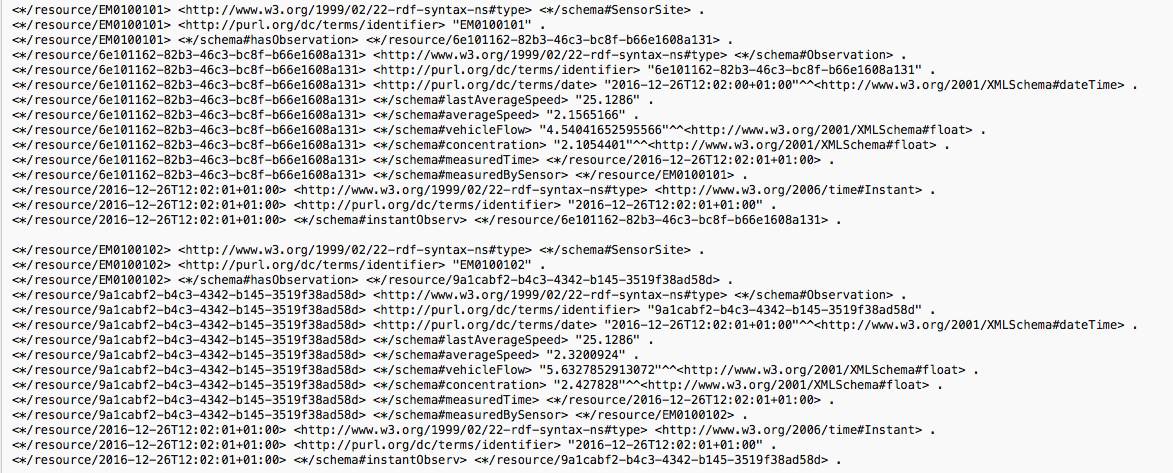
\includegraphics[height=5.5cm]{img/triplerdf2.png}
\caption{\emph{Esempio di un set di triple RDF (per motivi di rappresentazione grafica la stringa} \texttt{http://www.disit.org/km4city} \emph{è stata sostituita con *})}
\end{figure}

Nell'immagine d'esempio sono mostrate due simulazioni relative a due sensori distinti appartenenti alla solita classe (classe dei sensori del traffico). 
Ogni processo di simulazione genera un blocco di triple per ciascun sensore appartenente ad un set predefinito
risultato di un'interrogazione nella base dati RDF.
\subsection{Struttura delle Triple}
Ogni blocco di triple appartenente ad una stessa classe , come vedremo, ha la medesima struttura. Di conseguenza è stato possibile implementare un algoritmo in grado di valorizzare
i tre parametri della tripla che lo compongono (\emph{soggetto, predicato, oggetto}) in modo automatico a partire da alcuni parametri iniziali.\\
Il blocco di triple che descrivono il sensore è composto da: classi (o istanze), attributi della classe e riferimenti ad altre classi.\\
Nell'esempio di figura \ref{triplerdf} è riportato un blocco di triple suddiviso per classi. Ogni classe possiede obbligatoriamente l'attributo\\ \texttt{http://www.w3.org/1999/02/22-rdf-syntax-ns\#type} che identifica la classe alla quale appartiene quella risorsa.
Un altro attributo obbligatorio è \texttt{http://purl.org/dc/terms/identifier}. Il valore di questo attributo identifica l'id della risorsa della classe in questione.
Le altre triple della classe, infine, rappresentano proprietà della classe oppure sono riferimenti a risorse di altre classi.\\
\begin{figure}[!h]
	\begin{subfigure}{1\textwidth}
		\centering
		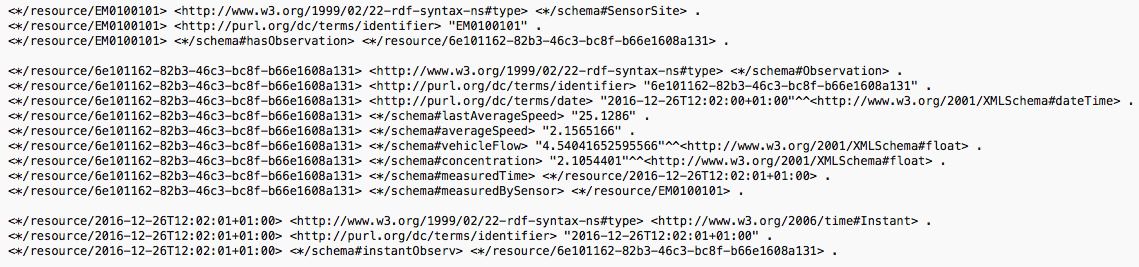
\includegraphics[width=14cm]{img/triple.png}
		\caption{Esempio di triple suddivise per classi RDF}\label{triplerdf}
	\end{subfigure}
	\begin{subfigure}{1\textwidth}
		\centering
		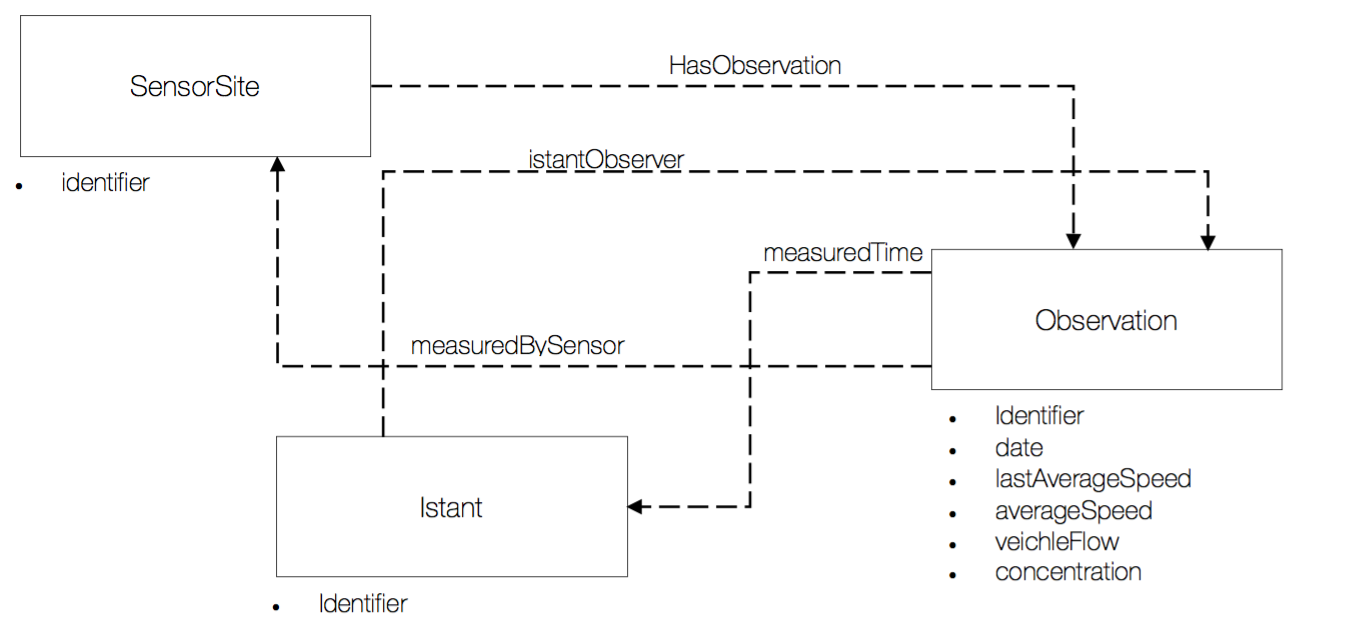
\includegraphics[width=14cm]{img/schema.png}
		\caption{Schema delle classi RDF riferite alle triple dell'esempio precedente}\label{schema}
	\end{subfigure}
	\caption{Triple e schema delle classi RDF}\label{rdfcombo}
\end{figure}
\newline
Nelle due immagini è mostrata la struttura di un esempio di triple RDF utilizzate per descrivere l'informazione relativa ad un sensore di traffico. Il tutto è composto da 3 classi ciascuna delle quali è identificata come una risorsa tramite un identificativo. Per ogni risorsa della classe, sono poi, specificati tutti i suoi attributi, mentre i riferimenti verso le altre classi (le frecce tratteggiate nello schema \ref{schema}) contengono come valore l'\emph{identifier} della risorsa alla quale fanno riferimento. 
\newpage

\section{Il File di Configurazione}
A fronte di quanto detto nel paragrafo precedente è stato implementato un algoritmo in grado di generare, in modo sistematico, una simulazione della campionatura in ordine ad un qualsiasi  sensore già definito all'interno dell'ontologia a partire da un file nel quale un utente esperto, cioè un utente che ha un'ampia conoscenza dell'ontologia di \emph{KM4City}, specifica come devono essere valorizzate le proprietà 
delle classi che definiscono il sensore. Tale file è scritto con la sintassi \emph{XML}.

\subsection{Struttura del file XML}
A seguito è descritta la struttura gerarchica dei nodi e delle loro proprietà che compongono il file di configurazione.\\

\begin{figure}[h!]
	\centering
	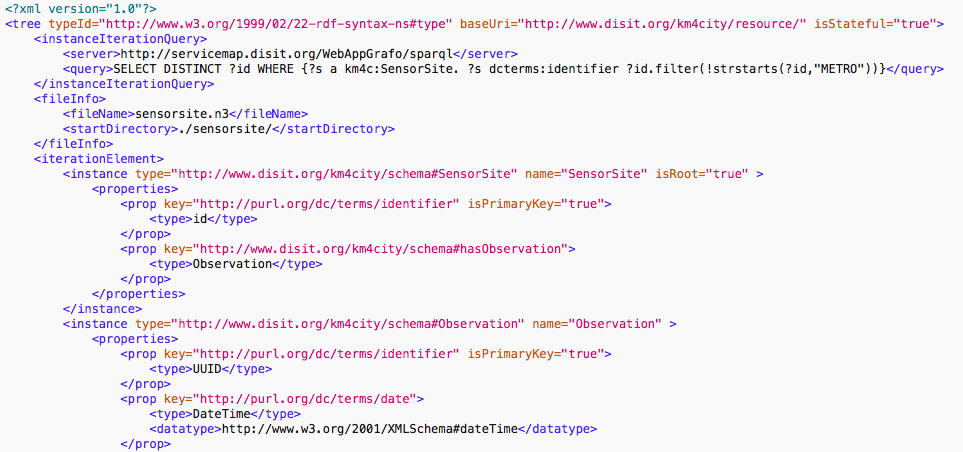
\includegraphics[width=14cm]{img/configxml.png}
	\caption{Estratto di un file di configurazione xml}\label{configxml}
\end{figure}

\subsubsection{<tree>}
\`E l'elemento radice ed ha le seguenti proprietà:
\begin{itemize}
	\item \textbf{typeId}: [Obbligatorio] Il suo valore indica l'\texttt{URI} da usare per indicare la tipologia della classe, ovvero, in altre, parole il valore del complemento della tripla 
	che deve indicare il tipo della classe.
	\item \textbf{isStateful} [Opzionale] Se true crea un file \emph{json} con tutti i valori dell'ultima esecuzione, tale file può essere riutilizzato in esecuzioni successive per tenere conto dei valori 
	precedentemente generati (le specifiche di questa funzionalità sono descritte a seguire nel paragrafo relativo alla tipologia \textbf{previusstate}). 
\end{itemize}
\subsubsection{<fileInfo>}\label{fileinfo}
Questo elemento definisce le specifiche del file di uscita, e deve contenere i seguenti elementi:
\begin{itemize}
	\item \textbf{FileName} [Obbligatorio] Specifica il nome del file \emph{.n3} d'uscita.
	\item \textbf{StartDirectory} [Obbligatorio] \`E la cartella all'interno della quale verranno generati i file risultato della simulazione.
\end{itemize}
A partire dalla cartella specificata sarà creata un'alberatura di cartelle con il seguente formato: \texttt{AAAA\_MM\textbackslash GG\textbackslash HH\textbackslash mmss\textbackslash filename.n3}, dove i simboli rappresentano i valori di data e e ora.


\subsubsection{<instanceIterationQuery>}
Questo elemento contiene  la definizione di una query SPARQL. Al suo interno si specifica la query SPARQ, i cui risultati rappresentano la lista di sensori sui quali iterare.
La query deve avere una struttura tale da restituire in uscita una lista di identificativi che rappresentano i sensori per i quali si vogliono generare delle simulazioni.\\
Questo elemento non possiede proprietà ma deve aver valorizzati i seguenti elementi:
\begin{itemize}
	\item \textbf{query} [Obbligatorio] Query sparql
	\item \textbf{server} [Obbligatorio] End-point a cui sottoporre la query
	\item \textbf{bindingValue} [Opzionale] Campo della select su cui andare a recuperare il valore d'uscita (default = id)
\end{itemize}

\subsubsection{<iterationElement>}
\`E l'elemento che contiene le definizioni della struttura RDF e le regole di generazione dei valori del sensore. Per ogni elemento generato dalla query si
rieffettua una generazione dei dati secondo le regole definite all'interno di questo elemento.\\
All'interno di questo elemento si definiscono quindi le istanze e le proprietà del sensore in accordo con la struttura della base dati RDF.\\
Questo oggetto contiene 2 tipologie di elementi:
\begin{itemize}
	\item \textbf{attributes} [Opzionale] Questo elemento contiene una lista di proprietà che non si riferiscono direttamente alla struttura RDF ma sono degli attributi 
	di supporto alla generazione dei valori delle proprietà del sensore. Talvolta può accadere che il valore di alcuni attributi sia il risultato di una combinazione di fattori la cui generazione 
	risulterebbe complicata se eseguita in una sola volta. L'idea che sta alla base dell'utilizzo di questa funzionalità è di poter demandare la generazione di quei valori, il cui risultato è funzione di più elementi,
	in questa sezione per poi referenziarli nella proprietà opportuna.\\
	Un caso emblematico in cui è utile dichiarare una variabile di appoggio in questa sezione, è quello in cui un valore sia funzione del risultato di una query e che in aggiunta debba subire elaborazioni successive. Per casi come questi, a meno che non sia possibile eseguire l'elaborazione del dato direttamente dalla query \texttt{SPARQL}, si può dichiarare in questa sezione una variabile che conterrà il risultato della query e nell'apposita proprietà (all'interno dell'istanza di cui fa parte) il valore verrà determinato attraverso una espressione, funzione della variabile che abbiamo dichiarato in questa sezione.
	\item \textbf{list<istance>} [Obbligatorio] Lista delle istanze che definiscono la struttura del sensore. In questa sezione si definiscono le istanze (rappresentanti le classi) e 
	le proprietà ad esse associate necessarie a definire l'intero oggetto (sensore) RDF. Le istanze contengono le informazioni necessarie a definire la tripla. Ognuna di esse contiene 
	una lista di proprietà dove per ognuna di esse sono definite oltre alle informazioni utili a generare la tripla anche le regole di generazione del valore del singolo attributo.
\end{itemize} 
\subsubsection{<istance>}
Elemento che definisce la struttura e gli attributi di un'istanza RDF.\\
Proprietà:
\begin{itemize}
	\item \texttt{type}: valore dell'uri \emph{rdf-syntax-ns\#type} dell'istanza.
	\item \texttt{name}: nome attribuito all'istanza utilizzato per richiamarla all'interno di altre istanze. 
	\item \texttt{isRoot}:se true indica se questa istanza contiene l'elemento su cui inserire il valore generato dalla query.
	\item \texttt{baseUri}: valore del \emph{baseURI} dell'istanza.
\end{itemize}
Elementi:
\begin{itemize}
	\item \textbf{properties} [Obbligatorio] Elemento che contiene la lista di attributi che definiscono l'istanza.
\end{itemize}
\subsubsection{<properties>}
Contiene la lista delle proprietà dell'istanza.
\begin{itemize}
	\item \textbf{list<prop>} [Obbligatorio]
\end{itemize}

\subsubsection{<prop>}
Con questo elemento si specificano le singole proprietà dell'istanza e come esse devono essere generate. Per ognuna di esse sono stati definiti dei campi utili alla generazione dei valori della tripla RDF ed altri campi necessari alla generazione del valore dell'attributo. Come vedremo in seguito sono stati individuati alcuni tipi con cui una proprietà può essere
definita. Ogni tipo necessita di ulteriori attributi definiti ad hoc per quella tipologia, utili alla generazione del valore di uscita.\\
Proprietà:
\begin{itemize}
\item \texttt{key}: valore della uri del predicato di quell'attributo.
\item \texttt{isPrimary}: se \emph{true} indica che quell'attributo è chiave primaria per l'istanza a cui appartiene (solo un attibuto per istanza può essere chiave primaria).
\end{itemize}
Elementi:
\begin{itemize}
\item \textbf{type} [Obbligatorio]: indica il tipo di valore che deve essere generato (ogni tipo può necessitare elementi aggiuntivi).
\item \textbf{uri} [Obbligatorio]: valore dell'oggetto della tripla RDF.
\item \textbf{format} : valore contenente la stringa con sintassi ''C-like'' del formato di uscita (e.g. ''\%.3f''). Il valore generato verrà dunque formattato in funzione della stringa definita all'interno dell'elemento.
\end{itemize}

\subsection{Lista Tipi}
La generazione dei valori può avvenire in molti modi: per cercare di offrire la maggiore capacità espressiva sono state implementate molteplici tipologie 
per la generazione pseudo-casuale dei valori delle proprietà.
Ognuno dei tipi sotto elencati può essere utilizzato come tipo di valore d'uscita per quella specifica proprietà.Sarà sufficiente specificarlo 
nell'attributo \emph{type} con a seguito i parametri di cui necessita.\\

\subsubsection{id}  Definisce che la proprietà dovrà contenere il valore proveniente dalla query di iterazione, 
questa proprietà deve essere attribuita all'istanza con \emph{isRoot = true}.\\
Parametri aggiuntivi: Nessuno
\subsubsection{integer} L'attributo restituirà un valore intero generato casualmente in un intervallo.\\
Parametri aggiuntivi:
\begin{itemize}
	\item \texttt{maxValue}: Estremo superiore dell'intervallo.
	\item \texttt{minValue}: Estremo inferiore dell'intervallo.
\end{itemize}
\subsubsection{float} L'attributo restituirà un valore float generato casualmente in un intervallo.\\
Parametri aggiuntivi:
\begin{itemize}
	\item \texttt{maxValue}: Estremo superiore dell'intervallo.
	\item \texttt{minValue}: Estremo inferiore dell'intervallo.
\end{itemize}
\subsubsection{md5} Genera il valore md5 di una stringa\\
Parametri aggiuntivi:
\begin{itemize}
	\item \texttt{md5String}: Contiene la stringa da crittografare
\end{itemize}
\subsubsection{datetime} 
Tipologia che genera una data in formato ISO 8601, se non specificati gli estremi dell'intervallo la data assume il valore dell'istante in cui è generata, altrimenti genera un valore casuale nell'intervallo di date.
Parametri aggiuntivi:
\begin{itemize}
	\item \texttt{maxValue}: Estremo superiore dell'intervallo.
	\item \texttt{minValue}: Estremo inferiore dell'intervallo.
\end{itemize}
\subsubsection{hourdependent} Questa tipologia serve a generare dei valori diversi per ogni ora della giornata in base a dei valori orari di riferimento specificati.
Parametri aggiuntivi:
\begin{itemize}
	\item \texttt{hourValue}: Contiene i valori di riferimento per ogni ora. Devono essere inseriti 24 valori separati da ';'. 
	\item \texttt{range}: Contiene il range di variazione all'interno del quale possiamo far variare il valore di riferimento indicato. Può essere un
	valore unico per tutti e 24 i valori oppure può essere definito in modo analogo a hourValue indicando i 24 valori del range.
\end{itemize}
\subsubsection{profiledependent} Con questa tipologia, che è concettualmente molto simile alla precedente, è possibile generare il valore di un attributo a partire da un set di profili normalizzati (tra 0 - 1) definiti per specifici giorni della settimana con
valori campionati ad intervalli di 15 minuti (96 campionature) che dovranno essere infine moltiplicati per un valore di riferimento. Questi valori sono specificati in file in formato \emph{.csv} che deve essere importato dal sistema.\\
\begin{figure}[!h]
	
	\begin{subfigure}{.3\textwidth}
		\centering
		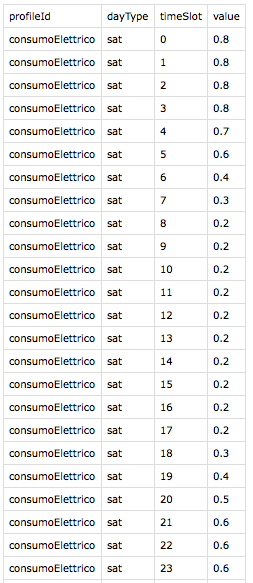
\includegraphics[width=.8\linewidth]{img/profilo1.png}
	\end{subfigure}
	\begin{subfigure}{.3\textwidth}
		\centering
		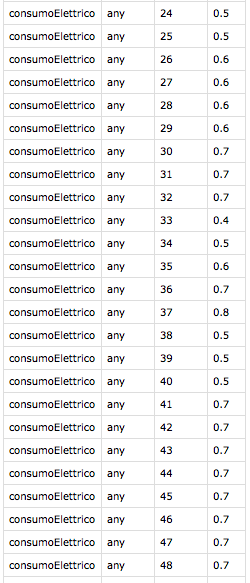
\includegraphics[width=.8\linewidth]{img/profilo3.png}
	\end{subfigure}
	\begin{subfigure}{.3\textwidth}
		\centering
		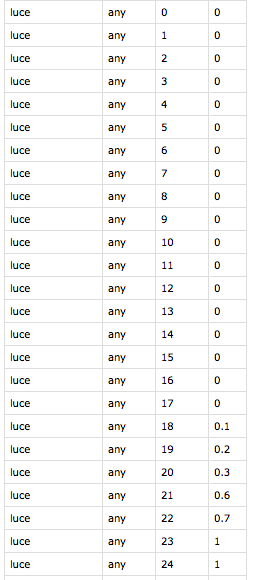
\includegraphics[width=.8\linewidth]{img/profilo2.png}
	\end{subfigure}
	\caption{Alcuni estratti del contenuto di un file \emph{.csv}}\label{csvfile}
\end{figure}
All'interno di un file \emph{.csv} possono essere definiti più di un profilo (e.g. ''consumo elettrico'', ''luce'', ''umidità''  ecc...) per ognuno di questi sono definiti i valori giornalieri di riferimento. La distinzione dei giorni può essere fatta specificando dei profili diversi per i diversi giorni della settimana oppure specificando un profilo \emph{any} valido per tutti i giorni per i quali non è definito un profilo. Come nel caso precedente anche qui dobbiamo definire un valore che specifica l'entità del rumore da aggiungere al valore di riferimento. Il valore finale è ottenuto quindi moltiplicando il valore ottenuto dal profilo in base all'orario per un valore di riferimento, tutto sommato con una perturbazione randomica di ampiezza specificata.\\
Parametri aggiuntivi:
\begin{itemize}
	\item \texttt{profilesFile} Contiene il nome del file \emph{.csv} da utilizzare
	\item \texttt{profileId} Indica quale è il profilo da considerare
	\item \texttt{maxValue} Valore base di riferimento 
	\item \texttt{variance} Valore della varianza 
\end{itemize}  

% esempio di file csv 

\subsubsection{fromset} 
Con questa tipologia si estrae un valore a caso da un set di elementi (se il set contiene un solo elemento sarà estratto sempre quello).
Parametri aggiuntivi:
\begin{itemize}
	\item \texttt{set} Lista di valori separati da ';'.
\end{itemize}
\subsubsection{query} Il valore dell'attributo è il risultato dell'esecuzione di una query (la query deve restituire un solo valore).\\
\newline
\emph{Elemento della stessa tipologia di \textbf{instanceIterationQuery}, con la sola differenza che in questo caso la query deve restituire un solo record e non una lista.}\\
\subsubsection{valueexpression} Definendo un attributo con questa tipologia si permette di definire il valore di un attributo come risultato di una espressione  algebrica o logica contenete variabili.\\
 Nel caso in cui si necessiti di calcoli più complessi rispetto ad una semplice espressione algebrica è possibile inserire del codice Javascript da far eseguire al sistema.
\\Parametri aggiuntivi:
\begin{itemize}
	\item \texttt{valueExpression} Contiene l'espressione algebrica o logica da eseguire. Le variabili devono essere dichiarate con la seguente sintassi \$\{nome\} dove nome è il valore inserito nelle proprietà dell'attributo prop
\end{itemize}
In caso di espressioni algebriche il valore restituito è sempre di tipo float.\\
Per una descrizione più approfondita delle variabili ed espressioni rgolari si rimanda al capitolo 3.3 .
\subsubsection{foregoing} Attraverso questa tipologia si può andare a referenziare il valore di una variabile generata in passi precedenti all'interno della stessa query di iterazione.\\
Lo scopo di questa tipologia è di permettere di referenziare all'interno di una iterazione un valore generato per un altro sensore sempre all'interno dello stesso ciclo di iterazione corrente.\\
Parametri aggiuntivi:
\begin{itemize}
	\item \texttt{defaultValue}: Valore da usare nel caso in cui l'attributo interessato non sia presente oppure non sia ancora stato generato.
	\item \texttt{refValue}:contiene la coppia \emph{iterazione - nomeVaribile} da cui prendere il valore. Il valore di iterazione può essere sia un intero, che rappresenta l'indice dell'iterazione 
	da cui prendere il valore, oppure l'id del sensore da cui prendere il valore interessato che viene specificato con la variabile nomeVariabile: il tutto con la sintassi \@[iterazione]\{nomeVariabile\}.
\end{itemize}
\subsubsection{previusstate}\label{previusstate} Questa tipologia ha un funzionamento simile alla precedente, con la differenza che in questo caso si può andare a referenziare valori generati in esecuzioni precedenti e non all'interno della stessa esecuzione.
Questa tipologia è utile per generare i valori di quegli attributi che hanno una dipendenza funzionale da stati precedentemente generati. Per fare in modo di poter utilizzare questa tipologia è necessario che sia settato a true la proprietà 
\emph{isStateful} nell'elemento \texttt{<tree>}. Così facendo il programma creerà un dump (in un file esterno in formato json) delle variabili generate ad ogni esecuzione in modo da poter recuperare il valore interessato e poterlo
utilizzare nell'iterazione corrente.
Parametri aggiuntivi:\\
\begin{itemize}
	\item \texttt{defaultValue}: Valore da usare nel caso in cui il valore interessato non sia presente oppure nel caso in cui non esista un'iterazione precedente a quella in oggetto.
	\item \texttt{refValue}:contiene la tripla \emph{indice - idSensore - nomeVaribile} da cui prendere il valore. L'\texttt{indice} specifica quale iterazione precedentemente generata si deve considerare (il conteggio avviene considerando l'iterazione corrente la 0 e la 1 quella precedentemente generata).
Ogni iterazione contiene una lista sensore; quindi è necessario specificare a quale sensore si fa riferimento tramite l'\texttt{idSensore} ed infine è necessario specificare il \texttt{nome} della proprietà che si vuole ottenere.
La sintassi da utilizzare per definire questa query di ricerca è la seguente: \#[indice][idSensore]\{nomeVariabile\}.\\
	\end{itemize}
	
\subsection{Variabili e Espressioni Algebriche}
Talvolta accade che i valori di alcune proprietà abbiano delle dipendenze funzionali da altri valori e che se ne debba tenere conto durante la fase di generazione.
I valori che sono generati per le proprietà delle classi sono valori estratti casualmente: anche se ne viene definito l'intervallo all'interno del quale variare, sono pur sempre valori casuali. 
Per quei valori che sono funzione di altri quindi deve essere introdotta una dipendenza dal valore generato casualmente.\\
Un esempio è il caso dei sensori dei parcheggi, i quali restituiscono informazioni sulle statistiche di utilizzo delle strutture. 

\begin{figure}[h!]
	\centering
	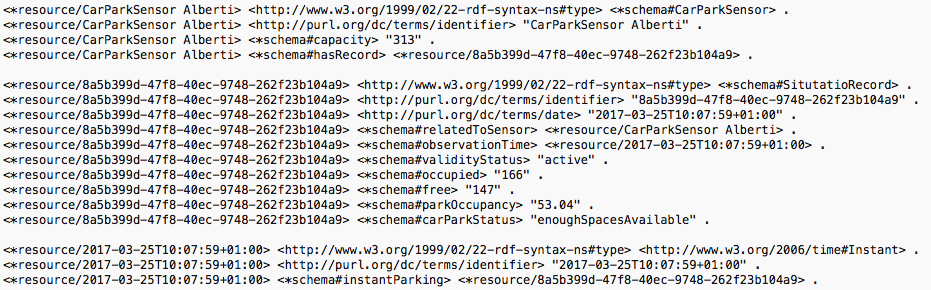
\includegraphics[width=14cm]{img/carParkSensor.png}
	\caption{Esempio di campionatura per un sensore di parcheggio}\label{carparksensor}
\end{figure}

Il valore principale che deve essere generato casualmente è il  ''\emph{numero di posti occupati}'', di conseguenza valori come \emph{numero di posti liberi} e \emph{percentuale di occupazione} devono essere funzione del valore casuale generato in precedenza.\\
Per risolvere questo tipo di problematiche è stata introdotta la possibilità di referenziare valori di proprietà già generati attraverso delle variabili e la possibilità di 
inserire espressioni algebriche.\\
Per ogni proprietà definita è necessario specificare un nome e per referenziare quel valore all'interno di altre proprietà si deve utilizzare la seguente sintassi: \$\{\emph{Nome\_Proprietà}\}
I valori nei quali è inserita una dipendenza funzionale saranno calcolati solo dopo aver generato tutte le loro dipendenze e nei casi in cui è necessario sarà possibile eseguire delle espressioni per determinare il valore di tali proprietà.
\newpage
\subsection{Esempio di file di configurazione}
Riprendendo l'esempio dei sensori di parcheggio citato nel paragrafo precedente, in questa sezione sarà mostrato un esempio del file di configurazione necessario per generare la simulazione relativa ad una campionatura di tale sensore (cfr. figura \ref{carparksensor}).

\begin{figure}[h!]
	\centering
	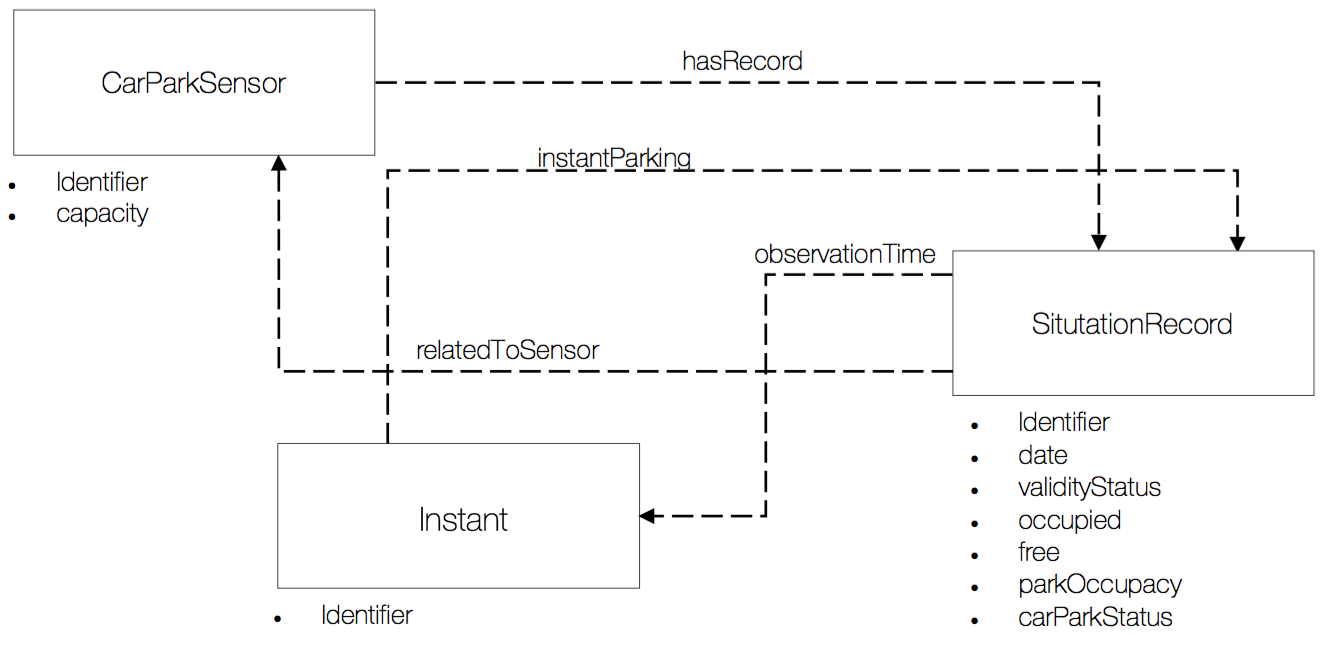
\includegraphics[width=14cm]{img/CPSschema.png}
	\caption{Schema delle classi RDF  dei sensori di parcheggio}\label{carparksensorschema}
\end{figure}
A partire dallo schema in figura il file \emph{.xml} per la generazione delle triple è il seguente:\\

\begin{figure}[h!]
	\centering
	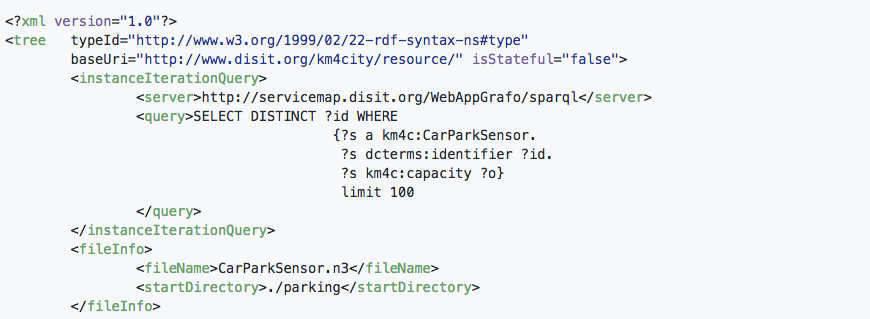
\includegraphics[width=14cm]{img/esempio_p1.png}
	\caption{Definizione della query di iterazione e de file di output}\label{esempio1}
\end{figure}
Nel \texttt{tree} si dichiarano rispettivamente la \texttt{uri} che conterrà il tipo dell'istanza e con \texttt{baseUri}, la stringa che definisce la prima parte del soggetto alla quale verrà aggiunto poi l'identificativo della risorsa. Per ogni istanza si può definire una \texttt{baseUri} diversa specificando tale attributo nella definizione dell'istanza (in caso contrario viene utilizzata quella specificata nel \texttt{tree}).
La proprietà \texttt{isStateful=''false''} specifica che queste simulazioni sono senza memoria.\\
\newline
All'interno dell'elemento \texttt{instanceIterationQuery} troviamo la definizione della query sulla quale si dovrà iterare. La query qui definita dovrà restituire sull'attributo \texttt{id} una lista di elementi che saranno l'identificativo delle risorse sulle quali verranno generate le simulazioni.\\
\newline
Nell'elemento \texttt{fileInfo} andiamo a definire la directory di partenza all'interno della quale creare le cartelle contenenti il file \emph{.n3} e il nome del file di uscita.\\
\newline
Finita la fase iniziale dove sono definite le informazioni generali si passa a specificare la struttura di ogni istanza, seguendo lo schema di figura \ref{carparksensor}. Per questa simulazione si devono definire tre istanze (\emph{CarParkSensor}, \emph{Instant} e \emph{SituationRecord}).\\
Le definizioni delle istanze sono inserite all'interno dell'elemento\\ \texttt{iterationElement}.\\
\begin{figure}[h!]
	\centering
	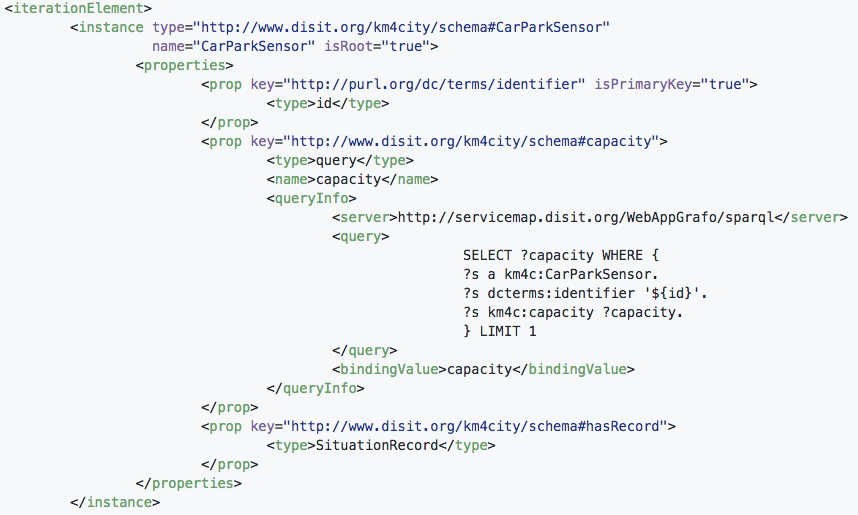
\includegraphics[width=14cm]{img/esempio_p2.png}
	\caption{Definizioni dell'istanza CarParkSensor}\label{esempio2}
\end{figure}
\newline
All'interno dell'elemento \texttt{instance} troviamo la definizione: dell'oggetto, il cui predicato identifica il tipo dell'istanza, del nome, dell'istanza e se questa istanza è \emph{root}.
A seguito troviamo la definizione di tutte le proprietà della classe (all'interno dell'elemento \texttt{properties}).
La prima proprietà definisce l'identificativo dell'istanza che essendo \emph{root} conterrà l'elemento estratto dalla query.\\
La seconda proprietà definisce l'attributo \emph{capacity} che rappresenta la capacità totale del parcheggio. Questo valore è ricavato tramite una query dove viene estratto il valore di capacità del sensore in oggetto. All'interno della query è stato inserito il carattere speciale \$\{id\}\footnote{La variabile \$\{id\}  insieme alla variabile \$\{index\} sono variabili di sistema e contengono rispettivamente l'id dell'iterazione corrente e l'indice dell'iterazione corrente} che contiene l'identificativo della risorsa nell'iterazione in corso.\\
Infine definiamo la proprietà \emph{hasRecord} che è un riferimento ad una istanza. Questa definizione viene fatta specificando nell'attributo \texttt{type} il nome dell'istanza a cui fare rifermento. Il valore restituito sarà il valore dell'identificativo di questa.
\newpage
\begin{figure}[h!]
	\centering
	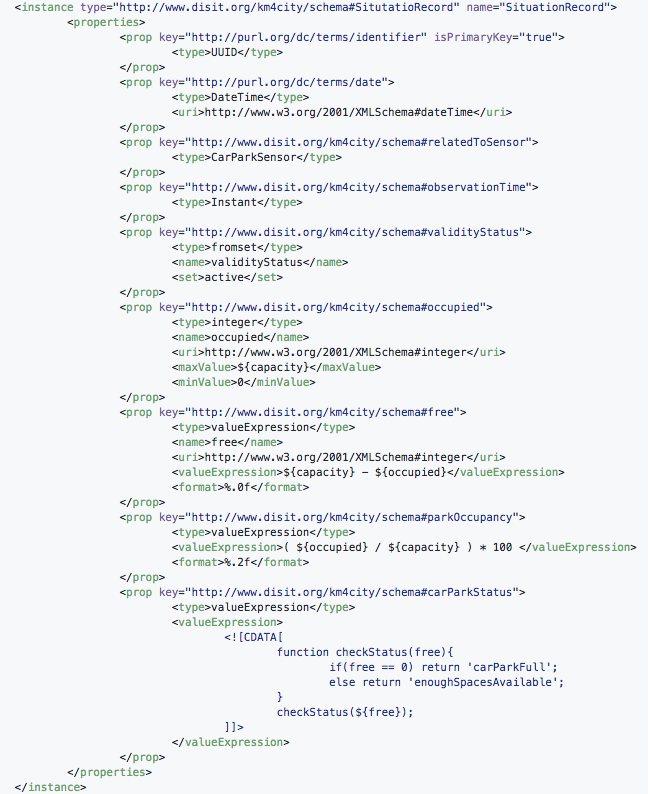
\includegraphics[width=14cm]{img/esempio_p3.png}
	\caption{Definizioni dell'istanza SituationRecord}\label{esempio3}
\end{figure}

In figura \ref{esempio3} è mostrata la definizione per l'istanza \emph{SituationRecord} con tutte le rispettive proprietà. In modo analogo al caso precedente anche in questo caso sono state definite la proprietà \texttt{identifier} e le proprietà che si riferiscono ad altre istanze (\texttt{Instant} e \texttt{CarParkSensor}) ed a seguito tutte le altre classi che definiscono questa istanza.\\
All'interno di questa istanza si fa un uso molto frequente di variabili ed espressioni (dovuto alla natura delle proprietà del sensore). Le variabili possono essere usate sia all'interno di espressioni regolari sia come parametri per la determinazione dei valori come nel caso della proprietà \texttt{occupied}, il cui valore deve essere un numero casuale tra 0 e il numero totale di posti di quel parcheggio (per ottenere questo valore si utilizza la variabile \$\{capacity\} che fa riferimento all'omonima proprietà definita nell'istanza precedente). \\
Per quanto riguarda le espressioni, di particolare interesse è la definizione di \emph{carParkStatus} dove al suo interno è stato definito del codice Javascript.\\
\newline
\begin{figure}[h!]
	\centering
	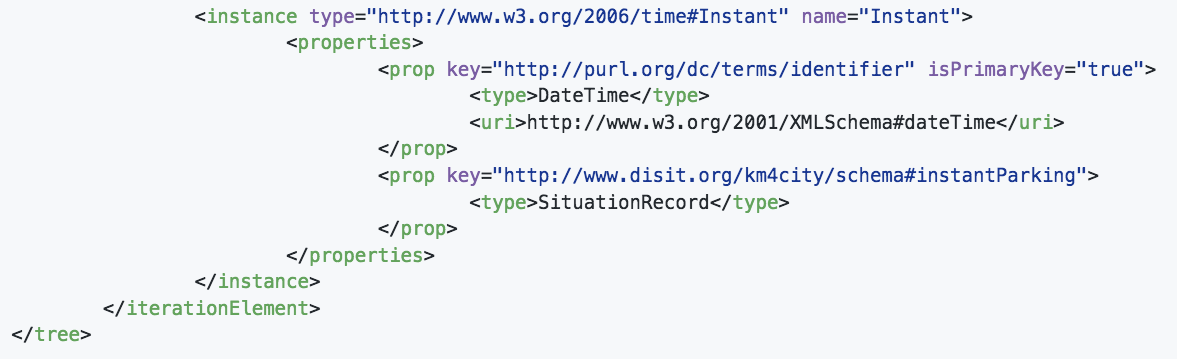
\includegraphics[width=14cm]{img/esempio_p4.png}
	\caption{Definizioni dell'istanza Instant}\label{esempio4}
\end{figure}
\newline
Infine in figura \ref{esempio4} è mostrata la definizione dell'istanza \emph{Instant} che completa la caratterizzazione di un sensore di parcheggio all'interno dell'ontologia di \emph{km4city}
\newpage
\section{L'applicativo Java}
Tutto il sistema descritto nei capitoli precedenti è stato realizzato attraverso un applicativo Java. A partire dal file di configurazione questo applicativo genera il file \emph{.n3} per KM4City. In questo capitolo saranno descritti i componenti principali che  compongono l'applicativo.\\
Il progetto è composto da 4 componenti principali:\\
\begin{enumerate}
	\item \emph{Main}. Classe principale, si occupa di avviare il processo di generazione della simulazione e scrivere i risultati su file.
	\item \emph{Classi per la gestione del dominio dei dati e dei formati}. In questo applicativo si parte da un informazione di base rappresentata in formato \texttt{XML}, inoltre ci sono altri due tipologie di formati che devono essere gestiti: \texttt{JSON e CSV}. Per ognuno dei formati sono state definite delle classi per la relativa gestione. 
	\item \emph{Classi del dominio applicativo}. Sono le classi che si occupano della definizione delle procedure applicative di alto livello.
	\item \emph{Classi per la gestione della simulazione generica}. Sono l'insieme delle classi implementate per poter astrarre dalla conoscenza degli aspetti delle diverse tipologie di dato definite e considerare le singole proprietà delle singole istanze come oggetti generici all'interno del processo iterativo di generazione delle triple.
\end{enumerate}
	\subsection{Main}
	Classe contenente il metodo omonimo che insieme alla classe \texttt{DataSimulator.java} si occupa: dell'acquisizione dei parametri iniziali, di fare partire il processo di generazione dei delle triple e di scrivere il file {.n3}. \\
	
	\texttt{java -jar sensorGenerator.jar -x sensor.xml -n simulazione\_parcheggi} \\
	
	Questa è la stringa con la quale viene lanciato il programma da linea di comando, sono necessari due parametri:\\
	\begin{enumerate}
		\item \texttt{-x} indica il file di configurazione xml (obbligatorio)
		\item \texttt{-n} nome della simulazione (opzionale)
	\end{enumerate}  
	
	La classe \texttt{main} valida gli argomenti passati in ingresso e successivamente istanzia un oggetto della classe \texttt{DataSimulator.java}.
	All'interno di quest'ultima si importa il file di configurazione all'interno di un oggetto e si da il via la processo di generazione delle triple, che una volta concluso se non si sono verificati errori, genera una stringa con tutte le triple. Una volta che questa è stata generata si crea (se non è già stato fatto) le cartelle utilizzando i valori di data e ora (cfr. capitolo \ref{fileinfo}). Infine viene creato il file \texttt{.n3}.\\
	\newline
	Nel caso di esecuzione con memoria (cfr. capitolo \ref{previusstate}) i file \texttt{.JSON} delle esecuzioni precedenti vengono importati in un'apposita lista al momento dell'importazione del file di configurazione e il file \texttt{.JSON} relativo all'iterazione corrente viene generato al termine dell'esecuzione nella solita cartella che contiene il file \texttt{.n3}.
	
	\subsection{Classi per la gestione del dominio dei dati e dei formati}
	All'interno di questo applicativo sono utilizzati tre tipologie di formati per l'interscambio di dati (\texttt{XML, JSON, CSV}), ognuno di essi utilizzato all'interno di un contesto diverso. Al fine di avere una gestione ottimale delle proprietà dei differenti formati, per ognuno di essi sono state definite delle classi che ne definiscono il comportamento.
	
	\subsubsection{XML}
	Questo formato è il formato utilizzato per definire il file di configurazione. Per gestire questo aspetto è stata definita la classe \texttt{Tree.java}, che contiene  la mappatura dei nodi della struttura del file \texttt{.xml}. Tramite questa mappatura un file \texttt{xml}, se rispetta la struttura definita, verrà serializzato all'interno di un oggetto di tipo \texttt{Tree} (figura \ref{treeClass}).\\
	\begin{figure}[h!]
		\centering
		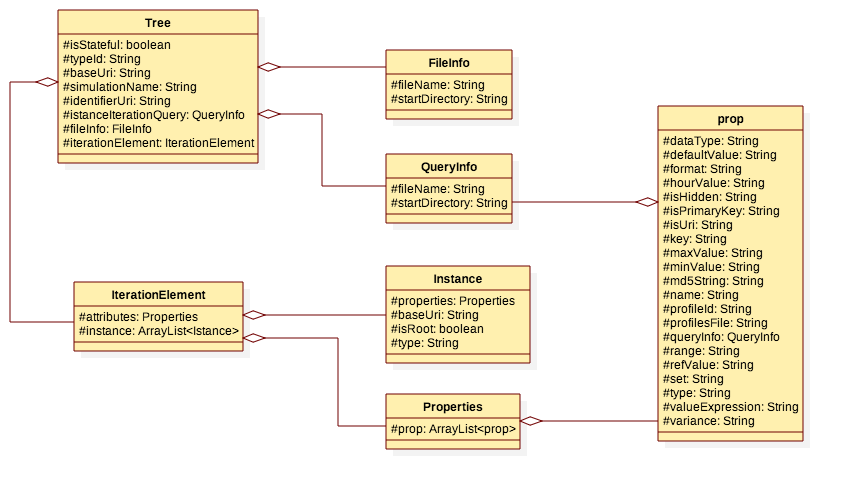
\includegraphics[width=14cm]{img/tree.png}
		\caption{Class Diagram della classe Tree}\label{treeClass}
	\end{figure}
	Per gestire i file di tipo \texttt{XML} è stata utilizzata la libreria esterna JAXB\footnote{Java Architecture for XML Binding (JAXB) - \url{https://jaxb.java.net}} che mette a disposizione le funzioni di serializzazione/deserilizzazione (Marshaller/Unmarshaller nel caso specifico di questa libreria) che sono utilizzate nella classe \texttt{XMLParsing.java} per importare un file in un oggetto di tipo \texttt{Tree}.
	
	\newpage
	\subsubsection{JSON} 
	Questo formato è utilizzato per gestire il caso dell'esecuzioni con memoria; se la proprietà \texttt{isStateful} del nodo \texttt{tree} è settata a \emph{true} si attiva la generazione dei file \texttt{JSON} contenti un \emph{dump} dell'esecuzione appena generata, ognuno di questi file viene salvato insieme al file \texttt{.n3} per poi essere importato all'interno di esecuzioni successive in modo da mettere a disposizione dell'esecuzione corrente anche lo stato assunto da esecuzioni precedenti.\\
	\begin{figure}[h!]
		\centering
		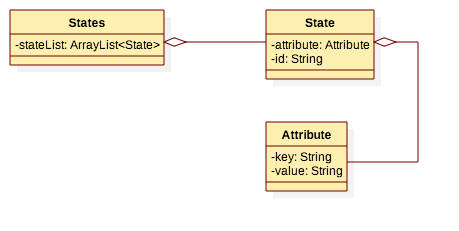
\includegraphics[height=5cm]{img/json.png}
		\caption{Class Diagram della classe per la gestione dei file json}\label{jsonClass}
	\end{figure}
	La classe \texttt{States} contiene 
	
	

\end{document}
%\subsection{Modellazione di Sistemi di Polling attraverso Reti di Petri Stocastiche}
%L'uso di reti di Petri stocastiche per la modellazione di Sistemi di Polling è volto ad ottenere una misura esatta delle performance su classi di sistemi in cui la popolazione è finita e il tempo di arrivo e il tempo di servizio assumono distribuzioni esponenziali.\\ Queste limitazioni possono essere superate utilizzando una \emph{phase-type expansion} per distribuzioni non esponenziali e si può emulare la popolazione infinita usando un elevato numero di gettoni\cite{fixedpoint}. Le reti di Petri stocastiche sono un modo di semplificare, risolvere e generalizzare modelli di Markov. Lo spazio degli stati del modello Markov risultante è tuttavia generalmente grande e tende ad esplodere con l'aumentare delle stazioni e degli utenti in coda, tanto che la memoria necessaria per analizzare la matrice contente la catena di Markov sottostante alla rete di Petri può superare la capacità disponibile anche per piccoli modelli. Di conseguenza, l'uso di catene di Markov per la soluzioni di sistemi reali risulta computazionalmente intrattabile o potrebbe richiedere tempi di calcolo molto lunghi\cite{pollingsys}.\\
%Per poter analizzare questa tipologia di problemi è necessario quindi operare qualche tipo di approssimazione, che, mantenendo un elevato grado di accuratezza, vada a diminuire notevolmente lo spazio degli stati della catena di Markov. Molti dei metodi proposti in letteratura operano delle riduzioni a partire dalla catena di Markov completa. Ciò comporta l'avere a disposizione la catena originale, la cui generazione e comunque un processo molto oneroso.\\ La soluzione proposta da Trivedi et. al. propone l'utilizzo di semplificazioni sulla struttura della rete di Petri in modo che la catena di Markov ad essa associata sia di dimensioni notevolmente ridotte.\\
%\newline
%Un sistema di Polling è dunque modellato come segue:\\
%\begin{figure}[!h]
%	\centering
%	\includegraphics[height=5.5cm]{img/sqss.eps}
%	\caption{\emph{Modellazione di un sistema di Polling a tre code con politica di selezione \textbf{Sequential} e politica di servizio \textbf{Single service}, dove la parte in alto rappresenta la struttura del server e 3 stazioni. Le code hanno un numero di gettoni finito che rappresenta la popolazione della coda, mentre il gettone in Polling0 è il gettone di controllo del flusso che cicla all'interno del server e regola il servizio delle diverse code.}}
%	\label{sqss}
%\end{figure}\\
%Con questa rete di Petri andiamo a modellare un sistema di Polling dove la politica di selezione della coda è di tipo sequenziale, cioè si servono le code in base al loro ordine, e la politica di servizio della coda prevede l'esecuzione di un singolo servizio. \\
%Le code hanno un numero di gettoni prefissato che rappresenta la popolazione massima che può avere la coda. All'interno delle code i gettoni  (con un tasso esponenziale $\lambda$ proporzionale al numero di gettoni in \emph{Idle})  passano dallo stato di inattività \emph{Idle} allo stato di attesa \emph{Waiting} rimanendo in quella posizione finché il server non passa a servire quella specifica coda.\\ Quando il server ha un gettone in \emph{Polling} e almeno un gettone in \emph{Waiting} si abilita la transizione \emph{Service} che con un tasso $\mu$ - rappresentativo del tempo di servizio - mette un gettone in \emph{Finish} e uno in \emph{Idle}.\\ Anche se i gettoni in \emph{Waiting} fossero più di uno ci sarebbe in ogni caso una sola esecuzione della transizione \emph{Service}, l'arco che collega la transizione \emph{Service} al posto \emph{Finish} fa in modo che sia eseguito un solo gettone. Infine, nel caso in cui si stia servendo una coda che non ha gettoni in attesa (un gettone in \emph{Polling} e zero in \emph{Waiting}) il server passa oltre quella coda tramite l'arco inibitore tra \emph{Waiting} e \emph{Complete} che abilita la transizione e mette il gettone per il controllo del flusso in \emph{Finish}, passando così alla coda successiva; il tempo di switch tra una coda e l'altra è modellato dalla transizione \emph{Select} di tasso $\gamma$.\\
%Per questi tipi di modelli di sitemi di Polling si posso calcolare vari misure delle performance come il \emph{Mean Cycle Time} (definito come il tempo medio per completare un intero ciclo, è il tempo necessario ad un gettone che parte da $Polling_i$ a tornare in quella posizione), oppure il \emph{Mean Response Time} (definito come il tempo medio  a partire dal quale un'istanza di un messaggio è generata finché questo non è trasmesso, cioè, il tempo che intercorre da quando un gettone aggiunto a \emph{Waiting} torna in \emph{Idle}). In questo elaborato abbiamo utilizzato come misura delle performance il \emph{Mean Response Time} calcolato come:
%\begin{equation}
%E[R_j] = \frac{M_j}{Tput(t_{Arrival_j})} - \frac{1}{\lambda_j}\;\; j \in\{1,2,..,N\} 
%\label{er1}
%\end{equation} 
%Dove $R_i$ rappresenta il tempo di risposta, $\lambda_i$ è il tasso di generazione di un messaggio e $Tput(t_{Arrival_j})$ è il throughput della transizione \emph{Arrival} della stazione $j$. Il throughput $Tput(t_{Arrival_j})$ si calcola moltiplicando la probabilità allo \emph{steady-state} di avere uno o più gettoni in \emph{Idle}: $\pi(Idle_j)$; per il tasso della transizione \emph{Arrival} $\lambda_j$.  
%\subsection{Politiche di selezione della coda}
%In questo elaborato sono state implementate ed analizzate varie politiche di servizio politiche di selezione della coda:
%\begin{itemize}
%	\item \textbf{Sequential} 
%	\item \textbf{Probabilistic proportional to queue length} 
%	\item \textbf{Probabilistic Proportional to Fixed Priority} 
%	\item \textbf{Uniform weight} 
%\end{itemize}
%I modelli di rete di Petri per queste diverse tipologie di selezione si dividono in due gruppi; \emph{sequenziale} o \emph{smart routing}. Il modello \emph{sequenziale} è quello visto in figura \ref{sqss}, mentre il modello \emph{smart routing} è quello mostrato di seguito in figura \ref{smartrouting}, con il quale è possibile implementare le altre tre politiche di servizio.
%\begin{figure}[!h]
%	\centering
%	\includegraphics[height=6.6cm]{img/smartrouting.png}
%	\caption{\emph{Questa rete di Petri rappresenta un un modello di Polling con politica di selezione della coda di tipo smart-routing, tramite questo modello si possono implementare varie politiche di selezione della coda che randomizzano la scelta della prossima coda da servire andando semplicemente a variare i parametri delle transizioni Select (in questo esempio la politica della coda è esaustiva).}}
%	\label{smartrouting}
%\end{figure}
%\paragraph{Sequential}
%Questa politica di servizio rappresenta il caso in cui le code sono servite secondo l'ordine con cui sono state inserite nel modello di Polling. L'esempio in figura \ref{sqss} mostra la struttura del server che è composto esclusivamente da interfacce di servizio verso le code collegate l'una all'altra.
%
%\paragraph{Probabilistic Proportional to queue Length} Con questa politica di servizio si vuole privilegiare le code che hanno un maggior numero di gettoni in attesa. La scelta sarà fatta in modo probabilistico con probabilità proporzionale al numero di gettoni in \emph{Waiting}. Il modello con reti di Petri è quello mostrato in figura \ref{smartrouting} dove la  transizione deterministica \emph{Select} ha per valore \emph{1+Waiting}. Con questa formula quando il gettone è in \emph{Ready} viene fatta una scelta probabilistica dando più peso alle stazioni con più gettoni in \emph{Waiting}. Una volta selezionata la coda questa eseguirà secondo la propria politica di servizio per poi restituire il controllo al sistema centrale, che successivamente sceglierà la successiva coda da visitare con lo stesso criterio.
%
%\paragraph{Probabilistic Proportional to Fixed Priority} Questa politica, tenta di simulare il caso in cui si hanno priorità fissate sulla transizioni che regolano l'accesso alle code. Con un sistema a priorità fissate su questo modello di Petri (figura \ref{smartrouting}) la scelta della prossima coda da servire ricadrebbe sempre su quella a priorità massima in quanto il gettone in \emph{Move} abilita tutte le transizione \emph{Select} delle interfacce e di conseguenza tra queste verrebbe scelta, sempre, quella a maggiore priorità. Per introdurre quindi un concetto di priorità che però non vada sempre ad escludere dalla scelta le code a minore priorità si utilizzando dei pesi fissi. Invece che definire un vettore delle priorità, si inserisce un vettore di pesi che andrà a pesare la probabilità di scelta delle varie code. Anche in questo caso il valore del peso della i-esima coda andrà a determinare il valore della transizione deterministica \emph{Select}. 
%
%\paragraph{Uniform Weight} Quest'ultima politica di selezione implementa il caso uniforme dove tutti i pesi delle varie code sono uniformi, cioè la probabilità di scelta della coda successiva è totalmente random.
%
%\subsection{Politiche di servizio}
%Le diverse politiche di servizio differiscono dal modo in cui le code gestiscono i gettoni, passano dallo stato di inattività allo stato di attesa e come essi devono essere eseguiti, prima di restituire il controllo al server.
%
%\begin{itemize}
%	\item \textbf{Single service} 
%	\item \textbf{Exhaustive} 
%	\item \textbf{K-Shots} 
%	\item \textbf{Only present at arrival}  
%\end{itemize}
%
%\begin{figure}[!h]
%	\begin{subfigure}{.33\textwidth}
%		\centering
%		\includegraphics[width=.8\linewidth]{img/sqss_q.png}
%		\caption{Single Service}
%		\label{fig:sqss_q}
%	\end{subfigure}%
%	\begin{subfigure}{.33\textwidth}
%		\centering
%		\includegraphics[width=.8\linewidth]{img/sqex_q.png}
%		\caption{Exhaustive}
%		\label{fig:sqex_q}
%	\end{subfigure}
%	\begin{subfigure}{.33\textwidth}
%		\centering
%		\includegraphics[width=.8\linewidth]{img/sqopks_q.png}
%		\caption{K-Shots / Only present}
%		\label{fig:sqopks_q}
%	\end{subfigure}
%	\caption{\emph{Nelle figure a,b,c sono mostrati i modelli di Petri delle varie politiche di servizio}}
%	\label{fig:queuePolicy}
%\end{figure}
%\paragraph{Single Service}
%La figura \ref{fig:sqss_q} mostra il caso già visto del singolo servizio, dove indipendentemente dai gettoni che trovo in attesa si esegue solo una volta il servizio e poi si restituisce il controllo al server.
%\paragraph{Exhaustive} La figura \ref{fig:sqex_q} mostra invece il caso della politica esaustiva, dove la coda esegue finché ci sono gettoni in attesa, ciò vuol dire che il numero di esecuzioni non è limitato dal numero di gettoni che trovo in attesa al momento della selezione della coda, perché nuovi gettoni possono arrivare in \emph{Waiting} anche durante il servizio, protraendo tale processo. Quest'ultimo si interromperà solo nel momento in cui non saranno più presenti gettoni in attesa. L'unica variazione nella rete rispetto al caso di servizio singolo è l'arco che dalla transizione \emph{Service} torna in \emph{Polling} (invece che andare in \emph{Finish}),. In questo modo dopo un'esecuzione della transizione \emph{Service} un gettone torna sempre in \emph{Polling} tenendo attiva la transizione \emph{Service} che esegue finché ci sono gettoni in \emph{Waiting}. Anche in questo caso è l'arco inibitore tra \emph{Waiting} e \emph{Complete} ad interrompere il processo di esecuzione della coda nel momento in cui non ci sono più gettoni in attesa.
%\paragraph{K-Shots \& Only present at Arrival} La figura \ref{fig:sqopks_q}, infine, mostra la modellazione del caso \emph{K-Shots} ed \emph{Only present at arrival}. I due casi rappresentano la situazione dove rispettivamente si eseguono un numero prefissato K di gettoni oppure si eseguono solo i gettoni che sono in attesa al momento della selezione della coda. Entrambi i casi sono simili perché al momento della selezione della coda si deve eseguire un numero deterministico di gettoni. Questa regola si realizza utilizzando una \emph{Marking update}, cioè un'aggiornamento della marcatura, che nel momento in cui la transizione \emph{Select} esegue, tramite un'opportuna funzione, modifica il numero di gettoni presenti nei vari posti riuscendo così ad implementare i due diversi casi:
%\begin{equation}
%\textbf{K-Shots} \begin{cases}Waiting=min(K,Arrived)\\Arrived=Arrived-min(k,Arrived)\end{cases}
%\end{equation}
%\begin{equation}
%\textbf{Only Present at Arrival}\begin{cases}Waiting=Arrived \\ Arrived=0\end{cases}
%\end{equation}
%Queste sono le \emph{Marking update} dei rispettivi casi che fanno in modo di eseguire un massimo di K gettoni, nel caso di \textbf{K-Shots} e solo i gettoni che sono in \emph{Arrived} al momento della selezione della coda, nel caso di \textbf{Only Present at Arrival}. In entrambi i casi si sposta un certo numero di gettoni da \emph{Arrived} a \emph{Waiting} e si aggiusta il numero di gettoni in \emph{Arrived}.\\ Una volta eseguiti tutti i gettoni in \emph{Waiting}, tramite l'arco inibitore si attiva la transizione \emph{Complete} che fa uscire dalla coda restituendo il controllo al server.
%\subsection{Sistemi di Polling asimmetrici}
%L'approssimazione tramite il metodo di punto fisso a differenza di altri tipi di semplificazioni come ad esempio il \emph{Folded-Model}\cite{fixedpoint}, vale anche nel casi in cui le stazioni siano, di tipo asimmetrico. Per asimmetrico si intende un sistema in cui le $N$ stazioni possiedono caratteristiche diverse l'una dall'altra.\\ 
%Le differenze tra le stazioni possono riguardare, in casi semplici, il numero di gettoni $M_i$ o il tasso di arrivo $\lambda_i$, oppure, in casi più complessi, le politiche di servizio. 
%In questo progetto si è ampliato la copertura dei casi possibili, dando la possibilità di creare modelli più possibile aderenti a quello che può essere un caso reale. Il sistema,    quindi, dà la possibilità di creare reti di Petri modulari dove la rete a $N$ stazioni, con una qualunque politica di selezione può essere composta da stazioni con politiche di servizio diverse e dotate di parametri distinti.
%\begin{figure}[h!]
%	\centering
%	\includegraphics[height=7.7cm]{img/mixed.eps}
%	\caption{\emph{Esempio di rete di Petri di un sistema di Polling asimmetrico a 3 code con politica di selezione \textquotedblleft smart routing\textquotedblright  e code di tipo Single Service, Exhaustive e K-Shots}}
%\end{figure}
%\newpage
%\section{Iterazione per Punto Fisso}
%\thispagestyle{plain}
%Con il metodo di iterazione di Punto Fisso andiamo a realizzare una rete di Petri che approssima la rete completa. Il metodo analizza in modo iterativo ogni stazione per determinare i parametri utili a simulare il comportamento del sistema completo, migliorando l'accuratezza ad ogni passo finché non è soddisfatto un qualche criterio di convergenza. \\ Il metodo propone di dividere il sistema originale a $N$ stazioni in 2 componenti: una rete di Petri che rappresenta la stazione che stiamo analizzando e un'altra rete di Petri che rappresenta le rimanenti $(N-1)$ stazioni.\\ L'idea che sta alla base di questa approssimazione è che nel momento in cui sto analizzando l'i-esima stazione (tipo, per un'analisi \emph{steady state}) posso considerare le rimanenti stazioni come un ritardo, cioè come il tempo che intercorre prima di tornare in quella stazione. Le $(N-1)$ stazioni, quindi, possono essere sostituite con una semplice transizione caratterizzata da un certo tempo di esecuzione che rappresenta il ritardo. Il processo iterativo è volto all'individuazione del vettore dei parametri che indicano il ritardo calcolato per ogni stazione.
%\subsection{Punto Fisso per reti sequenziali}
%A partire dunque da una rete di Petri completa che rappresenta un particolare modello di Polling,
%\begin{figure}[!h]
%	\centering
%	\includegraphics[height=5.8cm]{img/sqex.png}
%	\caption{\emph{Rete di Petri che modella il caso simmetrico con server \textbf{Sequential} e code \textbf{Exhaustive}}}
%	\label{sqex}
%\end{figure}\\
%\newpage
%la rete $S_i(N)$ che lo approssima ha questa struttura:
%\begin{figure}[!h]
%	\centering
%	\includegraphics[height=7.8cm]{img/apxsqex1.png}
%	\caption{\emph{Modello approssimato della rete in figura \ref{sqex}}}
%	\label{apxsqex}
%\end{figure}\\
%Il modello è stato ridotto ad una struttura con una singola stazione ed un \emph{server vacation}, rappresentato dal posto \emph{Approximate} e dalla transizione \emph{Delta}.
%Questo modello rappresenta l'approssimazione \textquotedblleft dal punto di vista\textquotedblright  della stazione \emph{i-esima} $i \in \{1,2,..N\}$.ll tasso $\delta$ della transizione \emph{Delta} modella il tempo che impiego nelle altre $N-1$ stazioni prima di tornare nella stazione \emph{i-esima}.
%Tramite l'approssimazione $S_i(N)$ calcoliamo ($\forall$ stazione $i$, ognuna con $M_i$ gettoni) il valore del \emph{Mean Response Time} relativo al nodo $i$ che servirà a determinare il vettore dei valori di $\delta_i$ da utilizzare nell'iterazione successiva
%\\In caso di modelli completamente simmetrici, in cui i la politica di servizio è uguale per ogni stazione e sono uguali sia i parametri $\lambda, \mu, \gamma$ sia il numero di gettoni per stazione, non è necessario calcolare un valore di $\delta$ per ogni stazione. Non vi è difatti differenza tra le code: il ritardo è uguale per tutte le code e con un unico valore di $\delta$ si riesce a modellare tutte le code. Nel caso, invece, di modello asimmetrico è necessario determinare il vettore dei  $\delta_i$ per ogni stazione.\\
%\newpage
%
%Definiamo\\
%$d_i \equiv$ \emph{mean delay} della stazione \emph{i-esima}\\
%$d_i(k) \equiv$  \emph{mean delay} della stazione \emph{i-esima} quando ci sono $k$ gettoni in coda\\
%$P(Waiting_i=k) \equiv$ la probabilità allo \emph{steady state}\footnote{Questo valore si ottiene tramite \emph{ORIS Tool} effettuando l'analisi steady state sulla rete di petri $S_i(N)$ con reward = \textquotedblleft If($Waiting_i=1,1,0$)\textquotedblright } di avere $k$ gettoni in coda nella stazione \emph{i-esima}\\
%$D_i \equiv$ somma dei ritardi di tutte le stazioni eccetto la stazione \emph{i-esima} \\
%$Tput(t) \equiv$ \emph{throughput} della transizione $t$\\
%
%Dove:\\
%\begin{equation}
%d_i = \sum_{k=0}^{M_i}d_i(k)\cdot P(Waiting_i = k)
%\label{di}
%\end{equation}
%\begin{equation}
%D_i = \sum_{j \in A,j\ne i}d_j \;,\; A=\{1,2,...,N\}.
%\label{Di}
%\end{equation}
%\begin{equation}
%\delta = \frac{1}{D_i}
%\label{delta}
%\end{equation}
%Il valore $d_i(k)$ rappresenta il tempo impiegato dalla stazione $i$ prima restituire il controllo al server. Questo valore può essere calcolato analizzando il seguente modello di Petri $T_i(k)$:
%\begin{figure}[!h]
%	\begin{subfigure}{.5\textwidth}
%		\centering
%		\includegraphics[height=5cm]{img/abs1.eps}
%		\caption{\emph{Single Service}}
%		\label{abs1}
%	\end{subfigure}
%	\begin{subfigure}{.5\textwidth}
%		\centering
%		\includegraphics[height=5cm]{img/abs2.eps}
%		\caption{\emph{K-Shots e  Only Present at Arrival}}
%		\label{abs2}
%	\end{subfigure}
%	\caption{\emph{Modello $T_i(k)$ per le varie tipologie di code}}
%\end{figure}\\
%Tramite questo modello vogliamo andare a determinare dopo quanto tempo ho un gettone in \emph{Finish} al variare di $k,\; k \in \{0,1,...,M_i\} $. \\ Per ottenere questo valore si utilizzano le seguenti formule: \\
%\begin{flalign}
%\textbf{Single Service}:\;	d_i(k) = \begin{cases} \frac{1}{\gamma} + \frac{1}{\mu}, & \mbox{se }k\mbox{ >0} \\ \frac{1}{\gamma}, & \mbox{altrimenti}\end{cases}
%\end{flalign}
%\begin{flalign}
%	\textbf{K-Shots}:\;	d_i(k) = \begin{cases} \frac{1}{\gamma} + \frac{1}{\mu} \cdot k, & \mbox{se }k\mbox{ $\le$ K} \\ \frac{1}{\gamma} + \frac{1}{\mu} \cdot K, & \mbox{altrimenti}\end{cases}
%\end{flalign}
%\begin{flalign}
%\textbf{Only Present at Arrival}: \; d_i(k) = \frac{1}{\gamma} + \frac{1}{\mu} \cdot k
%\end{flalign}
%In questo caso abbiamo semplificato i calcoli utilizzando come tempi impiegati dalle transizioni (a distribuzione esponenziale) il loro valore atteso.
%Per quanto riguarda invece il caso della politica di servizio \emph{Exhaustive} si deve utilizzare un modello diverso da quello visto in precedenza per ottenere il valore di $d_i(k$). Diversamente dai tre casi precedenti nel caso \emph{Exhaustive}, infatti, il numero di gettoni che ho al momento della selezione della coda può variare anche durante l'esecuzione (\emph{i.e.} ne possono arrivare di nuovi). Per questo motivo il modello visto in precedenza non vale per questo caso. \\ 
%Il modello $T_i(k)$ per il caso \emph{Exhaustive} è dunque: \\
%\begin{figure}[!ht]
%	\centering
%	\includegraphics[height=5.8cm]{img/abs3.eps}
%	\caption{\emph{Modello $T_i(k)$ per la politica di servizio Exhaustive}}
%	\label{ads3}
%\end{figure}\\
%Per calcolare $d_i(k)$ su questa rete di Petri occorre eseguire una \emph{Transient Analysis} con Reward = \emph{Finish} (utilizzando ORIS Tool). L'analisi mostra all'aumentare del tempo (campionato in intervalli discreti) la probabilità che ci sia uno o più gettoni in \emph{Finish}. Per ottenere dunque, una buona misura del tempo impiegato dalla coda ad eseguire il suo corso, in funzione di $k$, si prende come valore il tempo in cui la probabilità arriva ad una determinata soglia $\epsilon$ (generalmente molto alta).\\
%\newline
%A questo punto per ogni politica di servizio della coda si ha un modo per calcare il \emph{mean delay} $d_i(k)$ al variare di $k$. Questo valore è utilizzato nella (\ref{di}) per calcolare il tempo medio impiegato dalla coda $i$ per esaurire i sui gettoni (tempo medio di soggiorno nella coda $i$). Nella (\ref{di}), infatti si moltiplica il tempo medio di soggiorno quando ci sono $k$ gettoni in attesa per la probabilità di avere $k$ gettoni in attesa, ottenendo il tempo medio di soggiorno nella coda. Infine dopo aver calcolato i $d_i \; \forall \;i  \in \{1,2,...,N\}$ è possibile calcolare con la (\ref{Di}) il tempo che occorre prima di tornare nella coda $i$, utilizzato successivamente come misura del \emph{server vacation} per l'iterazione al passo successivo.\\
%
%\begin{algorithm}
%	\caption{Algoritmo \emph{Mean Response Time} iterativo basato sul metodo di Punto Fisso}
%	\label{fixedpoint}
%	\begin{algorithmic}[1]
%		\For{$i=1\; \textbf{to}\; N$}
%			\For{$k=0\; \textbf{to}\; M_i$}
%				\State solve $T_i(k)$ to get $d_i(k)$
%			\EndFor
%			\State $\delta_i^{(0)} \gets d_i(N)$ /* initial value of $\delta$ */
%		\EndFor
%		\Repeat
%			\For{$i=1\; \textbf{to}\; N$}
%				\State set $\delta_i^{(m)}$ in $S_i(N)$ model
%				\For{each $k$}
%					\State get $P(P_{Waiting} = k)$ and compute $d_i$ as equation (\ref{di})
%				\EndFor
%			\EndFor
%			\For{$i=1\; \textbf{to}\; N$}
%				\State compute $D_i$ as equation (\ref{Di})
%				\State compute $\delta_i^{(m+1)}$ as equation (\ref{delta})
%			\EndFor
%		\Until{$(|\delta_i^{(m+1)} - \delta_i^{(m)}| < \epsilon)$}
%		\State compute $E[R_i]$ as equation (\ref{er})
%	\end{algorithmic}
%\end{algorithm}
%
%L'iterazione va avanti finché ci sono variazioni significative nei valori di $\delta_i$, tra un'iterazione e l'altra. Si calcola, infine, il \emph{Mean Response Time} della coda $i$ come:
%\begin{equation}
%E[R_i] = \frac{M_i}{Tput(t_{Arrival_i})} - \frac{1}{\lambda_i}
%\label{er}
%\end{equation} 
%\paragraph{Esistenza ed unicità della soluzione} Il funzionamento descritto si basa sull'esistenza della soluzione e sull'unicità della stessa, così come efficacemente dimostrato dal lavoro di K.S. Triveti \emph{et al}\cite{fixedpoint} che segue.
%Quest'ultima mostra l'esistenza per il \emph{Mean Cycle Time} di un sistema simmetrico.\\
%\newtheorem{brower}{Teorema}
%\begin{brower}{\textbf{Teorema di punto fisso di Brower\\}}
%	Sia $ \mathbb{R}^n $ spazio n-dimensione di reali. Se esiste un insieme compatto e convesso $S \subset \mathbb{R}^n$ ed esiste una funzione continua $f$ tale che $f(x) \in S\;,\;  \forall x \in S$, allora esiste una soluzione all'equazione $f(x) = x$.   
%\end{brower}
%Si considera quindi un modello $S_i(N)$ di un sistema di Polling simmetrico dove $\lambda_i = \lambda$, $\mu_i = \mu$, $\delta_i = \delta$ e $\gamma_i = \gamma$ per tutte le stazioni.\\
%\newline
%Definiamo\\
%$d\equiv$  il ritardo medio di una stazione\\
%$D\equiv$ il tempo medio per attraversare $(N-1)$ stazioni\\
%$E[C]\equiv$ \emph{mean cycle time} del sistema di Polling\\
%$Tput(t)\equiv$ il throughput della transizione $t$\\
%$\pi(p)\equiv$ \emph{steady state probability} di avere uno o più gettoni nel posto $p$\\
%Allora\\
%\begin{equation*}
%E[C] = \frac{1}{Tput(Select_i)} = N \times d
%\end{equation*}
%\begin{equation*}
%D = (N- 1)d = (N - 1)\times\frac{E[C]}{N}
%\end{equation*}
%\begin{equation*}
%= \frac{N -1}{N} \times \frac{1}{Tput(Select_i)}
%\end{equation*}
%E sia $D = 1/\delta$,
%\begin{equation*}
%\delta = \frac{N}{N -1} \cdot Tput(Select_i)
%\end{equation*}
%$Tput(Select_i)$ è definito come:
%\begin{equation*}
%Tput(Select_i) = \gamma \cdot \pi(Finish_i)
%\end{equation*}
%\begin{equation}
%\delta = \frac{N}{N -1 }\cdot \gamma\cdot\pi(Finish_i)
%\label{deltafp}
%\end{equation}
%$\pi(Finish_i)$ può essere rappresentato come:
%\begin{equation}
%\pi(Finish_i) = \frac{\frac{1}{\gamma}}{\{\frac{1}{\mu}\cdot\pi(Waiting_i)+0(1-\pi(Waiting_i))\}+\frac{1}{\delta}+\frac{1}{\gamma}}
%\label{finish}
%\end{equation}
%$\pi(Waiting_i)$ è in relazione con $\pi(Finish_i)$, \emph{i.e. ,} $\pi(Waiting_i) = \phi(\pi(Finish_i))$ per una qualche funzione $\phi$. Così $\pi(Finish_i)$ può essere rappresentata come una funzione $f$, di se stessa come segue:
%\begin{equation}
%\pi(Finish_i) = \frac{\frac{1}{\gamma}}{\frac{1}{\mu}\cdot\phi(\pi(Finish_i))+\frac{1}{\delta}+\frac{1}{\gamma}} = f(\pi(Finish_i))
%\label{fp}
%\end{equation}
%Sia $x= \pi(Finish_i)$ e sia $S = [0,1]$ un insieme compatto. Allora $x$, la probabilità \emph{steady state} di avere un gettone in $Finish_i$, è in $S$. Dati $1\setminus\mu$, $\pi(Waiting_i)$, $1\setminus\gamma$, e $1\setminus\delta$ numeri reali non negativi,
%\begin{equation*}
%f(x) = \frac{\frac{1}{\gamma}}{\frac{1}{\mu}+\phi(x)+\frac{1}{\delta}+\frac{1}{\gamma}} =  \frac{\frac{1}{\gamma}}{\frac{1}{\mu}+\pi(Waiting_i)+\frac{1}{\delta}+\frac{1}{\gamma}} \in [0,1]
%\end{equation*}
%e $f$ è una funzione continua. Questo vuol dire che $f(x) \in S \; \forall x \in S$.\\
%\newline
%Adesso è necessario mostrare la convessità. Un insieme $S \subset \mathbb{R}^n$ è convesso se
%\begin{equation*}
%ax + (1-\alpha)y = z \in S \; \; \forall x,y \in S, \; \alpha \in [0,1]
%\end{equation*}
%Dati $x,y \in [0,1]$ e $\alpha \in [0,1]$, segue che $z$ è anch'essa in [0,1] . Quindi $S$ è un insieme compatto e convesso e $f$ è continua. Quindi c'è una soluzione all'equazione,
%\begin{equation*}
%f(x) = x \;\;tale\; che\;\; x, \; f(x) \in S
%\end{equation*} 
%Siccome esiste un punto fisso per $x$ \emph{i.e.,} $\pi(Finish_i)$, esiste anche un punto fisso per $\delta$ della (\ref{deltafp}). Di conseguenza c'è una soluzione di punto fisso per il \emph{mean cycle time}: 
%\begin{equation*}
%	E[C] = \frac{N}{(N-1)\delta}
%\end{equation*}
%Attraverso questa si riesce a dimostrare l'esistenza del punto fisso per il \emph{Mean Cycle Time} per un modello di Polling simmetrico. Allo stesso modo è possibile dimostrare l'esistenza del punto fisso per il \emph{Mean Response Time} e per sistemi asimmetrici. 
%\subsection{Punto Fisso per reti non sequenziali}
%Quanto visto fino ad adesso si riferisce a sistemi di Polling in cui la politica di selezione della coda è di tipo sequenziale. Tale aspetto permette di sommare i singoli ritardi dovuti alle code per ottenere il tempo di ciclo. Per sistemi nei quali la politica di servizio non è sequenziale (\emph{Probabilistic Proportiona to Queue Length, Simulate Priority e Uniform Weights}) utilizzare la somma dei singoli ritardi delle code, per determinare il tempo di ciclo, non è corretto. Per questo motivo è stato necessario trovare un nuovo modo per determinare il $D_i$ (somma dei ritardi di tutte le stazioni eccetto la stazione \emph{i-esima}). Tramite questo metodo è possibile riutilizzare l'algoritmo iterativo (\ref{fixedpoint}) visto in precedenza, effettuando solo delle piccole varianti per il calcolo di $D_i$.\\
%Per quanto si sia cercato di rimanere il più aderenti possibile al lavoro di riferimento\cite{fixedpoint}, per il quale è garantita l'esistenza della soluzione, per questa variante del problema manca la dimostrazione analitica dell'esistenza del punto fisso e pertanto non è garantita la convergenza del processo.\\
%\newline
%Lo schema di un sistema di Polling con politica di selezione della coda non sequenziale è quello visto nel capitolo precedente in figura \ref{smartrouting}. Questa particolare struttura fa sì che non ci sia un tempo di ciclo deterministico, in quanto un gettone può visitare la solita coda anche più volte consecutivamente. Le formule viste in precedenza  per la determinazione del $\delta$, quindi, non sono più valide.\\ Per risolvere il problema si utilizza un modello di rete di Petri  $R_i(N)$ che approssima la rete reale come segue:
%\begin{figure}[!ht]
%	\centering
%	\includegraphics[height=5cm]{img/sojournTime.eps}
%	\caption{\emph{Modello per il calcolo del tempo medio di ciclo}}
%	\label{sojourn}
%\end{figure}\\
%La rete in figura \ref{sojourn} rappresenta la rete per il calcolo del tempo di ciclo per la stazione 1, i posti $p_1,p_2,p_3$ rappresentano le 3 stazioni e le transizioni deterministiche $sojourn_2,sojourn_3$ modellano il tempo di permanenza nelle stazioni attraverso il valore $d_i$ calcolato come dalla (\ref{di}).\\
%La transizione immediata $Select_i$ infine, modella (attraverso dei pesi $w_i$) le modalità di selezione della coda, che variano a seconda della politica. \\
%\newline
%Siano, $N_i = \sum_{k=0}^{M_i} k\cdot P(Waiting_i)$ il \# atteso di gettoni che trovo nella stazione $i$ quando ci torno e $p_i$ il vettore delle priorità prefissate;
%\begin{table}[ht!]
%	\centering
%	\begin{tabular}{ccc}
%		\hline
%		Prob. Proportional to queue length & PR Fixed Priority & Uniform Weight \\ \hline
%		$w_i = 1 + N_i$      & $w_i = p_i$  & $w_i = 1$               \\ \hline
%	\end{tabular}
%	\caption{\emph{Determinazione dei pesi $w_i$ in base alla politica di selezione}}
%	\label{weights}
%\end{table}\\
%Costruendo opportunamente il modello $R_i(N)$ con i parametri $d_i$ e $w_i$ si riesce a trovare per ogni stazione il tempo $D_i$ necessario per la determinazione del valore di $\delta_i$. Il tempo di ciclo $D_i$ si ottiene eseguendo una \emph{regenerative transient analisys} sulla rete tramite \emph{ORIS Tool}. Questa analisi calcola al variare del tempo quanto è la probabilità di avere uno o più gettoni in $p_i$.\\
%\begin{figure}[ht!]	
%	\centering
%	\includegraphics[height=5.8cm]{img/transient.png}
%	\caption{\emph{Grafico della regenerative transient analysis con reward = $p_i$}}
%	\label{transient}
%\end{figure}\\
%Il valore di $D_i$ è determinato dal tempo in cui la probabilità si attesta ad un valore vicino a uno.\\
%Attraverso questo procedimento non è necessario modificare l'algoritmo iterativo (\ref{fixedpoint}), ma basta delegare alla tipologia di \emph{server} il calcolo di $D_i$.
%\newpage
%\section{ORIS Tool}
%\thispagestyle{empty}
%Questo elaborato è stato realizzato utilizzando il progetto \emph{ORIS Tool}, un progetto realizzato dal Software Science and Technology Lab, Department of Information Engineering, University of Florence. ORIS Tool è un applicativo desktop cross-platform per l'analisi di STPNs dotato di interfaccia grafica. \\
%\begin{figure}[ht!]
%	\centering
%	\includegraphics[height=11cm]{img/oris.png}
%	\caption{\emph{Esempio dell'interfaccia grafica di ORIS Tool}}\label{oris}
%\end{figure} \\
%L'editor grafico permette di gestire e costruire modelli di Petri a partire dai componenti principali (posti, transizioni, gettoni, ecc.) e grazie all motore di analisi di ORIS è possibile effettuare operazioni come \emph{Regenerative Transient Analisys} e \emph{Steady State Analysis}.\\
%Oltre a ciò questo progetto mette a disposizione una libreria Java SIRIO, che permette di creare Reti di petri e di effettuare su di esse tutte le tipologie di analisi offerte da ORIS\cite{oris}.
%\begin{figure}
%	\centering
%	\includegraphics[height=7cm]{img/sirio1.png}
%	\caption{\emph{UML component diagram di ORIS Tool}}\label{sirio}
%\end{figure}\\
%\begin{figure}
%	\centering
%	\includegraphics[height=7cm]{img/sirio2.png}
%	\caption{\emph{Diagramma di un oggetto PetriNet della libreria SIRIO}}\label{sirio2}
%\end{figure}\\
%\newpage
%\section{Progetto}
%\thispagestyle{plain}
%Questo progetto consiste in un applicativo Java che utilizza la libreria SIRIO, capace di realizzare l'approssimazione di una rete tramite l'iterazione di punto fisso. Questa applicazione a partire da parametri che definiscono la struttura del sistema di Polling reale (\#code,tipologia di code, \# di gettoni per coda, ecc.) calcola il vettore dei parametri $\delta_i$, necessari ad approssimare il sistema reale tramite la rete $S_i(N)$ di figura \ref{apxsqex} (un valore di $\delta$ diverso per ogni coda nel caso di code asimmetriche) e restituisce come output l'errore commesso dall'approssimazione sulla valutazione di alcune \emph{performance} rispetto al modello completo.\\ L'applicativo, in sostanza, implementa l'algoritmo iterativo descritto nel capitolo precedente per tutte le varianti di servizio e di selezione della coda.
%\newline
%\begin{figure}[ht!]
%	\centering
%	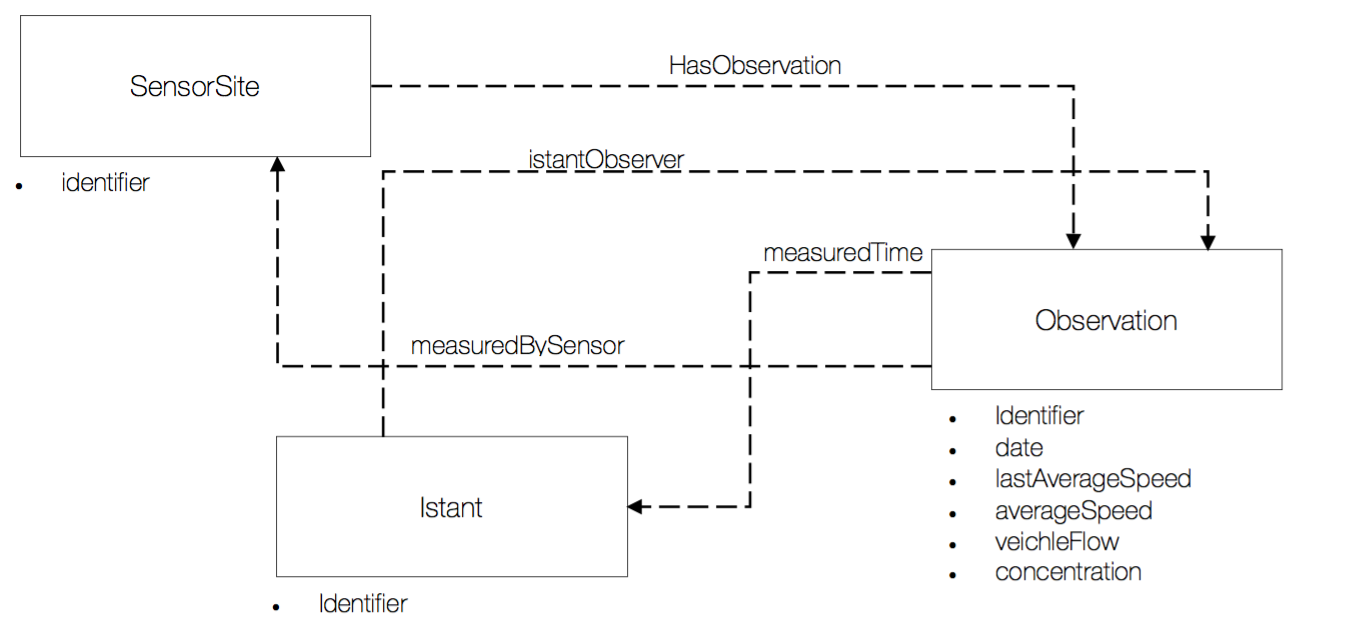
\includegraphics[width=13cm]{img/schema.png}
%	\caption{\emph{Schema generale dell'applicazione}}
%\end{figure}
%\ \\
%\newline
%Partendo dai parametri inseriti, il \emph{builder} dell'applicazione è in grado di costruire una rete di Petri che modella un sistema di Polling modulare e asimmetrico e la corrispettiva rete $S_i(N)$ che lo approssima, per poi determinare i parametri $\delta_i$ con l'algoritmo iterativo. Un sistema di polling modulare e asimmetrico  è un sistema modellato da una rete di Petri, che implementa una qualsiasi combinazione di tipologia di server e tipologia di code in cui le code possono differire l'una dall'altra sia per tipologia sia per i parametri che la descrivono.\\
%\newpage
%Il progetto è composto da 4 componenti principali: 
%\begin{enumerate}
%	\item \emph{Main}. Rappresentato dalla classe \texttt{PollingRunner.java} si occupa di acquisire i parametri per la definizione del modello, lanciare il \emph{builder}, lanciare il processo iterativo e raccogliere i risultati.
%	\item \emph{Classi per la gestione dei moduli di reti di Petri}. La caratteristica principale di questo applicativo è la possibilità di generalizzare il modello approssimato astraendo dalle diverse politiche di selezione e di coda. Per riuscire a mantenere questo elevato livello di astrazione è necessario implementare un complesso sistema di interfacce per la creazione delle reti di Petri e gestione delle operazioni da eseguire su di esse.
%	\item \emph{Classi per la gestione delle transizioni}. Oltre all'intercambiabilità delle politiche e la totale asimmetria dei parametri che definiscono il sistema di Polling per aumentare la capacità descrittiva del sistema è stata implementata anche la possibilità di poter scegliere la tipologia di transizioni che andranno a descrivere il comportamento del sistema. Essendo le transizioni i componenti fondamentali dell'analisi iterativa, si è resa necessaria l'implementazione di un opportuno sistema per la gestione della fase di definizione della rete e per la gestione delle operazioni.
%	\item \emph{FixedPointModel}. Questa classe, a partire dai paramatri inseriti, crea tutte le reti di Petri necessarie e implementa il processo iterativo di punto fisso.
%	
%\end{enumerate}
%\subsection{Main}\label{cap:main}
%La classe che contiene il metodo \texttt{main} è la classe \texttt{PollingRunner.java}. Questa classe, per prima cosa, si occupa di acquisire i parametri necessari alla definizione della rete per la quale si vuole creare l'approssimazione. Successivamente alla validazione dei parametri si occupa di lanciare il \emph{builder} per la creazione dei modelli e del lancio del processo iterativo per poi raccogliere i risultati e confrontarli con il sistema reale.\\
%L'acquisizione dei parametri può essere fatta attraverso due modalità: da linea di comando o tramite l'importazione di un file \emph{.ini} contenete i parametri.\\ Le due modalità sono state realizzate per dare la possibilità ad un eventuale utente finale di differenziare l'esecuzione a seconda del contesto, in quanto la modalità da linea di comando, se pur più verbosa come vedremo in seguito, si presta molto per contesti iterativi  (\emph{e.g.} all'interno di script \emph{shell} o \emph{python}) dove è necessario effettuare molteplici prove al variare di alcuni parametri, o più in generale in contesti \emph{machine-machine}.\\
%\begin{figure}[ht!]
%	\centering
%	\includegraphics[width=14cm]{img/linea.png}
%	\caption{\emph{Descrizione dei parametri da inserire da linea di comando}}\label{linea}
%\end{figure}\\
%Il metodo con il file di configurazione, invece, si propone per casi di esecuzioni singole, o più in generale, per contesti dove l'interazione è di tipo \emph{human-machine}, in cui la definizione dei parametri risulta di più facile comprensione per l'utente.
%\begin{figure}[ht!]
%	\centering
%	\includegraphics[width=14cm]{img/ini.png}
%	\caption{\emph{Esempio di file .ini}}\label{ini}
%\end{figure}
%In figura \ref{ini} è mostrato il contenuto del file di inizializzazione contenete la lista dei parametri, nel formato chiave-valore, necessari a definire un sistema di Polling. Come vedremo poi, molti dei parametri sono espressi sotto forma di vettori. Questi servono a descrivere gli aspetti ed il comportamento di ogni singola coda in quanto si deve poter essere in grado si poter descrivere ogni coda tramite parametri diversi.\\
%\newline
%\begin{enumerate}
%	\item \texttt{Server:} indica la politica di selezione della coda.
%	\item \texttt{Queue:} è un vettore della solita dimensione del numero di code e specifica la politica di ognuna delle code.
%	\item \texttt{numQueue:} indica il numero di code del sistema.
%	\item \texttt{Tokens:} contiene il vettore dei token, indica il numero di token che deve avere ogni coda coda.
%	\item \texttt{Prio:} è il vettore delle priorità simulate ha la solita dimensione del numero di code. Le code con politica \emph{Probabilistic Proportional to Fixed Priority} avranno come priorità il corrispettivo valore del vettore. 
%	\item \texttt{Lambda:} è il valore del \emph{firing rate}  utilizzato insieme al valore di $\rho$ per determinare tasso $\lambda_i$ della transizione \emph{Arrival} come da equazione (\ref{ro}).
%	\item \texttt{rho:} vettore dei valori di \emph{offered load}. Per ognuno dei valori viene eseguito il processo iterativo.
%	\begin{equation}
%	\rho = \sum_{i=1}^{N} \frac{M_i\cdot\lambda_i}{\mu}
%	\label{ro}
%	\end{equation}
%	\item \texttt{K:} vettore dei valori di K per le code con politica \emph{K-Shots}.
%	\item \texttt{mu-gamma-delta:} sono le definizioni delle tre transizioni $\mu,\gamma,\delta$. Gli attributi devono contenere il tipo di transizione (EXP,UNI,DET) e i parametri necessari per descriverla
%\end{enumerate}
%Il file di inizializzazione come altre opzioni relative all'esecuzione del programma devono essere definite da linea di comando dai comandi:
%\begin{enumerate}
%	\item \texttt{-ini <outFile>}: questa flag indica che vogliamo che le impostazioni siano acquisite dal file \emph{outFile.ini} (se non specificato il file di default è \emph{model.ini}).
%	\item \texttt{-o <outFile>}: tramite questa opzione si può chiedere al programma di redirigere l'output anche su un file di testo.
%	\item \texttt{-showInfo}: questa flag abilita la stampa a video dei risultati anche durante la fase di elaborazione intermedia (non influisce sulla stampa dei risultati finali).
%	\item \texttt{-debug}: abilita la modalità debug nella quale il processo viene interrotto, in attesa della pressione di un tasto, in tutti i passaggi intermedi dell'iterazione. 
%\end{enumerate}
%Volendo eseguire il programma utilizzando il file \emph{.ini} di figura \ref{ini}; un esempio di esecuzione da riga di comando è il seguente:\\
%\newline
%\texttt{java -jar fixedPoint.jar -ini -o output.txt -showInfo}\\
%\newline
%equivalentemente senza utilizzare il file \emph{.ini} lo stesso risultato si ottiene:\\
%\newline
%\texttt{java -jar fixedPoint.jar -sPolicy SQ -qPolicy SS,SS,SS,SS,SS\\ 
%\quad -numQueue 5 -rho 0.1,0.2,0.3,0.4,0.5,0.6,0.7,0.8,0.9 \\
%\quad -t 1,1,1,1,1 -l 2,1,1,1,0.5  -o output.txt}\\
%\newline
%Il programma creerà, quindi, una rete sequenziale con 5 stazioni tutte a singolo servizio con un token per stazione e la sua approssimazione, confrontando infine i risultati ottenuti dall'iterazione per punto fisso per ogni valore di $\rho$.
%\subsection{Classi per la gestione dei moduli di reti di Petri}
%All'interno di questo progetto è necessario avere delle implementazioni tali da permettere di creare reti di Petri modulari utilizzando la libreria SIRIO. Per modulare si intende un sistema di Polling a $N$ stazioni, in cui a partire da una qualsiasi politica di selezione le stazioni possono avere politiche e parametri distinti. L'implementazione di queste classi è stata necessaria al fine di mantenere un alto grado di generalità del codice, cioè senza dover specificare un comportamento per ogni singola combinazione dei parametri.\\
%Per prima cosa si nota che la struttura di un sistema di Polling con reti di Petri è tale da poter permettere una intercambiabilità tra le varie politiche in quanto tutte le diverse strutture presentano le medesime caratteristiche.\\
%\begin{figure}[ht!]
%	\centering
%	\includegraphics[height=4.5cm]{img/sqss1.png}
%	\caption{\emph{Moduli di un sistema di Polling}}\label{modules}
%\end{figure}
%\ \\
%In figura \ref{modules} sono mostrati i moduli di cui è composto un sistema di Polling realizzato con reti di Petri. Come si nota dalla figura ci sono 3 componenti principali: il \emph{server}, le \emph{service interface} (una per coda), e le \emph{code}. Indipendentemente dalla tipologia di server e di coda, quindi, è stato possibile realizzare un processo di costruzione della rete basato sulla gestione dei 3 diversi moduli (qualsiasi siano le politiche inserite dall'utente).\\
%La struttura di questo meccanismo si basa sulla definizione di tre classi astratte che regolano come i tre componenti devono interfacciarsi tra di loro per costruire la rete di Petri.\\
%\begin{figure}[ht!]
%	\centering
%	\includegraphics[height=8cm]{img/domain.eps}
%	\caption{\emph{Class Diagram delle classi del dominio}}
%\end{figure}
%Ogni classe che specializza le classi astratte- \emph{server, service, queue}- ridefinisce i metodi astratti definiti nelle classi generiche andando ad implementare tali metodi secondo le proprie caratteristiche.\\
%Questo meccanismo permette di definire un unico metodo di costruzione della rete di Petri che risulta indipendente dalla particolare combinazione di politiche di selezione e servizio scelte dall'utente.\\
%Le classi \texttt{Server} e \texttt{Queue} hanno entrambe un metodo statico non astratto necessario a determinare il tipo. Di seguito ne vediamo il codice per la classe \texttt{Server} (per la classe \texttt{Queue} il funzionamento è il medesimo).
%\newpage
%\begin{figure}[h]
%	\centering
%	\includegraphics[width=14cm]{img/getserver.png}
%	\caption{\emph{Acquisizione dell'oggetto Server}}\label{getserver}
%\end{figure}
%\ \\
%A partire dall'oggetto \texttt{serverType}, dal quale, in base alla politica scelta dall'utente si riesce a ricavare il nome della classe corrispondente, si costruisce una istanza dell'oggetto di una delle classi che specializzano la classe \texttt{Server}. Il nuovo oggetto è istanziato con un costruttore generico a partire dai parametri passati (che per semplicità sono i soliti per ogni tipologia di classe). Per ognuno di essi si estrae il tipo ed insieme agli stessi parametri lo si passa al costruttore generico che istanzierà un oggetto della classe richiesta.\\ 
%Gli altri metodi, tutti dichiarati astratti, riguardano il calcolo dei valori come $d_i$ e di $D_i$ i quali a seconda della tipologia di Server/Coda avranno un procedimento di calcolo distinto (come descritto nei capitoli precedenti) e di conseguenza ogni tipologia dovrà definire il suo.
%\subsection{Classi per la gestione delle transizioni}
%In questo elaborato è stata implementata la possibilità di modificare la tipologia di alcune transizioni al momento dell'inizializzazione della rete. Anche in questo caso si è voluto mantenere un elevato grado di astrattezza delegando ai livelli inferiori della struttura la singola gestione delle diverse tipologie. Utilizzare varie tipologie di transizioni permette di avere un quadro più ampio circa il comportamento della rete: difatti, a parità di rete ma con tipologie di transizioni diverse, si possono ottenere risultati anche molto diversi tra di loro.\\
%\newline
%Le tipologie tra le quali è possibile scegliere sono: 
%\begin{enumerate}
%	\item \emph{Exponential}
%	\item \emph{Deterministic}
%	\item \emph{Uniform}
%\end{enumerate}
%Le tre tipologie in sostanza vanno a determinare dopo quanto tempo la transizione esegue (dal momento in cui viene abilitata).  Nel primo caso il tempo è determinato secondo una probabilità che ha una distribuzione esponenziale con un certo tasso $\lambda$. Nei due rimanenti casi i tempi di esecuzione sono determinati rispettivamente: da un valore deterministico associato alla transizione nel caso \emph{Deterministic} e da un valore scelto a caso all'interno di un'intervallo anch'esso definito dall'utente nel caso \emph{Uniform}.
%Come già definito precedentemente (cfr. par. \ref{cap:main}), le definizioni delle tre transizioni per le quali è possibile modificare la tipologia sono: a) $\gamma_i$  è la transizione che regola il tempo di switch tra una stazione e la successiva; b) $\mu_i$ è la transizione che regola i tempi di servizio sui gettoni in attesa; c) $\delta$ è la transizione del \emph{Server Vacation} che simula le $N-1$ stazioni nel modello approssimato. Ognuna di queste tre può essere di uno qualsiasi dei tre tipi definiti sopra.
%\begin{figure}[ht!]
%	\centering
%	\includegraphics[height=5cm]{img/transitionManager.eps}
%	\caption{\emph{Class Diagram delle classi per la gestione delle transizioni}}
%	\label{transitionmanager}
%\end{figure}		
%Utilizzare questo meccanismo ci permette di non preoccuparci ad alto livello di come ogni singola tipologia gestisca i vari aspetti: i calcoli specifici sono delegati alle classi che specializzano la classe astratta \emph{TransitionManager}. Gli oggetti di questa classe sono istanziati in modo analogo ai casi di \texttt{Queue} e \texttt{Server} visti in precedenza, dove tramite la \emph{reflection} si crea l'oggetto della classe desiderata.
%\subsection{FixedPointModel}
%La classe \texttt{FixedPointModel.java} infine è la classe che, a partire dai parametri iniziali ed utilizzando le strutture precedentemente definite, permette di costruire i modelli tramite reti di Petri necessari per l'esecuzione del processo iterativo di punto fisso.
%Questa classe si basa su tre componenti (oggetti) principali:
%\begin{enumerate}
%	\item \texttt{PollingModel} - è l'oggetto che si occupa della gestione della rete di Petri che modella il sistema reale.
%	\item \texttt{ApproximateModel} - questo oggetto contiene la struttura per la gestione dei modelli approssimati $S_i(N)$.
%	\item \texttt{MeanDelayModel} - questo è l'oggetto che gestisce i modelli $T_i(k)$.
%\end{enumerate}
%\begin{figure}[ht!]
%	\centering
%	\includegraphics[height=8cm]{img/fixedPoint.eps}
%	\caption{\emph{Class Diagram delle classi per la gestione dei modelli di Petri }}
%	\label{fixedPoint_cd}
%\end{figure}
%Come si nota dal diagramma delle classi di figura \ref{fixedPoint_cd} l'oggetto \texttt{PollingModel} contiene una singola rete di Petri, mentre gli oggetti \texttt{ApproximateModel} e \texttt{MeanDelayModel} contengono una lista di reti di Petri. Questo perché la struttura dei modelli $S_i(N)$ e $T_i(k)$ varia al variare della tipologia di stazione, quindi i due oggetti dovranno avere tante reti di Petri quante sono le stazioni del modello reale.\\
%Per ogni modello è stato definito un metodo \texttt{build()} necessario alla costruzione di quella specifica rete di Petri. La struttura della rete però varia a seconda della particolare combinazione di tipologia di selezione e tipologia di coda servizio; grazie alla particolare implementazione generica dei moduli che compongono un sistema di Polling, con un unico metodo si riesce a costruire una qualsiasi combinazione scelta dall'utente.\\
%\begin{figure}[ht!]
%	\centering
%	\includegraphics[width=14cm]{img/build.png}
%	\caption{\emph{Costruzione della rete di Petri per il modello di Polling reale}}\label{build}
%\end{figure}\\
%Questo metodo costruisce la rete composta da un server ad $N$ code. La costruzione avviene passo-passo: per prima cosa si crea l'oggetto server, poi ciclando sul numero di code, si inserisce una per volta l'interfaccia di servizio (il service) e la coda, assegnando ad ogni passaggio i parametri definiti per quella coda.\\
%Inizialmente le code, i service e il server sono dichiarati utilizzando le rispettive classi generiche: saranno i metodi \texttt{getServer()} e  \texttt{getQueue()} a restituire il tipo giusto in base alle scelte dell'utente. Dato quindi il tipo di server questo in base al numero di code aggiungerà un service ed una coda (dei tipi opportuni) alla propria struttura. La coda, infine, si occuperà anche di collegarsi al service.\\Il collegamento coda-service è delegato alla coda in quanto ogni tipologia di coda ha un suo modo specifico di collegarsi al services. L'operazione è eseguita dal metodo \texttt{linktoService(PetriNet,Service)}.\\
%\begin{figure}[h!]
%	\begin{subfigure}{.5\textwidth}
%		\centering
%		\includegraphics[width=.8\linewidth]{img/block1.eps}
%		\caption{}
%	\end{subfigure}%
%	\begin{subfigure}{.5\textwidth}
%		\centering
%		\includegraphics[width=.8\linewidth]{img/block2.eps}
%		\caption{}
%	\end{subfigure}
%	\caption{\emph{Collegamento tra code e service nel caso di server sequenziale}}
%	\label{linktoservice}
%\end{figure}\\
%\begin{figure}[h!]
%	\begin{subfigure}{.5\textwidth}
%		\centering
%		\includegraphics[width=.8\linewidth]{img/block3.eps}
%		\caption{}
%	\end{subfigure}
%	\begin{subfigure}{.5\textwidth}
%		\centering
%		\includegraphics[width=.8\linewidth]{img/block4.eps}
%		\caption{}
%	\end{subfigure}
%	\caption{\emph{Collegamento tra code e service nel caso di server smart service}}
%	\label{linktoservice2}
%\end{figure}\\
%In figura \ref{linktoservice} ci sono due casi distinti di collegamento tra coda e server (sequenziale): il collegamento è composto da 3 archi uno dei quali è un arco inibitore. L'arco da \emph{Polling} a \emph{Service} e l'arco inibitore da \emph{Waiting} a \emph{Complete} sono fissi per ogni tipologia di coda mentre la destinazione dell'arco uscente da \emph{Service} varia a seconda della politica. Infatti, se la coda è di tipo \emph{Single Service} (figura \ref{linktoservice}.a) è necessario collegare \emph{Service} a \emph{Finish} mentre negli altri tre casi (\emph{Exhaustive, K-Shots} e \emph{Only Present at Arrival}) anche se la struttura della coda varia il collegamento con il service è il medesimo (figura \ref{linktoservice}.b): l'arco uscente da \emph{Service} va sempre in \emph{Polling}.\\
%Nella struttura del service dei server di tipo \emph{smart}, figura \ref{linktoservice2},manca il posto \emph{Finish}: nei casi in cui le code sono \emph{Exhaustive, K-Shots} o \emph{Only Present at Arrival} non ci sono problemi (figura \ref{linktoservice2}.b) ma in caso di coda \emph{Single Service} l'arco che da \emph{Service} dovrebbe andare in \emph{Finish} è sostituto da un arco che da \emph{Service} va in \emph{SelectNext}. Per regolare questo tipo di collegamento nei \texttt{Service} di server di tipo \emph{smart} nel valore di \emph{Finish} è settato il riferimento al posto \emph{SelecNext}. Così facendo il metodo \texttt{service.getFinish()} restituirà il posto opportuno dove collegare l'arco.\\
%\newline
%In modo analogo a quanto visto i metodi \texttt{build()} delle classi \texttt{ApproximateModel} e \texttt{MeanDelayModel} costruiscono gli $N$ modelli $S_i(N)$ e $T_i(k)$ ed il metodo \texttt{fixedPointIteration()} implementa il processo iterativo descritto dall'algoritmo \ref{fixedpoint}. Anche all'interno di questo metodo sono utilizzate le classi generiche in modo da delegare i calcoli alle classi specializzate a seconda dei casi.\\ 
%L'uscita dal processo iterativo si ha né momento in cui uno o più valori di $\delta$ non subiscono delle variazioni significative, cioè $|\delta_i^{(m)} - \delta_i^{(m-1)}|<\epsilon$  è vera per qualche valore di $i, i \in \{1,2,..,N\}$ con $\epsilon=0.001$.\\
%A fine del processo si valuta l'errore calcolando il \emph{Mean Response Time} (equazione \ref{er}) sia per il modello approssimato che per il modello completo. 
%L'errore $E$ è definito da:
%\begin{equation*}
%E = \frac{100\times(approximate\;model\; -\; real\;model )}{( real\;model)}
%\end{equation*}
%Le performance sul \emph{Mean Response Time} e l'errore relativo $E$ sono calcolati per ogni valore del parametro $\rho$ dove:
%\begin{equation}
%\rho = \sum_{i=1}^{N} \frac{M_i\cdot\lambda_i}{\mu} 
%\label{error}
%\end{equation}
%Fissato $\rho$ e dato il vettore dei $c_i$\footnote{È il vettore lambda richiesto in input, serve a proporzionare i tassi di arrivo} dove $\lambda_i = c_i\cdot \lambda$  allora:
%\begin{equation*}
%\lambda = \frac{(\mu\cdot\rho)}{\sum_i M_i \cdot c_i}
%\end{equation*}
%Per cui il variare del valore di $\rho$ va ad alterare il tasso $\lambda$ con cui i gettoni arrivano in \emph{Waiting}.
%Questo meccanismo di alterazione è utilizzato come perturbazione sui parametri del modello.
%\newpage
%\section{Risultati}
%\thispagestyle{plain}
%In questa sezione mostriamo i risultati ottenuti dal sistema, tali risultati vanno a confrontare i valori ottenuti dal \emph{Mean Response Time} (equazione \ref{er1}) sia per il sistema di Polling completo che per la sua approssimazione tramite il modello $S_i(N)$. Il confronto si ottiene tramite il calcolo delle errore come nella (\ref{error}).
%Se non diversamente specificato i valori di $\mu, \gamma$ sono i soliti utilizzati nel lavoro di K.S. Trivedi \emph{et. al.}\cite{fixedpoint} (transizioni esponenziali di tasso $\mu=1.25$ e $\gamma=294.12$).\\ Di seguito sono riportati i risultati ottenuti al variare di alcuni parametri raggruppati in base alla politica di selezione della coda.\\
%\begin{table}[ht!]
%	\centering
%	\scriptsize
%	\begin{tabular}{ll}
%		\hline
%		\multicolumn{2}{c}{Policy}                                                     \\ \hline
%		\multicolumn{1}{c}{Server}                      & \multicolumn{1}{c}{Queue}    \\ \hline
%		SQ = Sequential                                 & SS = Single Service          \\ \hline
%		PR = Probabilistic Proportional to Queue Length & EX = Exhaustive              \\ \hline
%		FP= Probabilistic Proportional to Fixed Priority                         & OP = Only Present at Arrival \\ \hline
%		UF = Uniform Weight                             & KS = K-Shots                 \\ \hline
%	\end{tabular}
%\end{table}
%\subsection{Sequential}
%\ \
%\begin{table}[hb!]
%	\begin{minipage}[b]{0.48\linewidth}\centering
%	\centering
%		\caption{\scriptsize \emph{Server=SQ, Queue=[SS,SS,SS], Token=[3,3,3], $\lambda$=[2,1,0.5]}}
%		\label{tab1}
%	\tiny
%	\begin{tabular}{c c c c c}
%		\hline
%		$\rho$ & Queue & $S_i(N)$ & Polling Sys & error \\ \hline
%		0.1 & SS & 0.8764276 &   0.8766610    & 0.03\% \\
%		0.1 & SS & 0.8833974 &   0.8835492    & 0.02\% \\
%		0.1 & SS & 0.8871805 &   0.8870385    & 0.02\% \\ \hline \hline
%		0.2 & SS & 0.9544951 &   0.9559966    & 0.16\% \\
%		 0.2 & SS & 0.9672650 &   0.9681787    & 0.09\%  \\
%		 0.2 & SS & 0.9746365 &   0.9743347    & 0.03\% \\ \hline \hline
%		 0.3 & SS & 1.0430463 &   1.0454060    & 0.23\% \\ 
%		 0.3 & SS & 1.0599672 &   1.0609508    & 0.09\% \\
%		 0.3 & SS & 1.0702866 &   1.0684791    & 0.17\% \\ \hline \hline
%		 0.4 & SS & 1.1438409 &   1.1452686    & 0.12\% \\
%		 0.4 & SS & 1.1626796 &   1.1618288    & 0.07\% \\
%		 0.4 & SS & 1.1747907 &   1.1689575    & 0.50\% \\ \hline \hline
%		 0.5 & SS & 1.2587054 &   1.2556921    & 0.24\% \\
%		 0.5 & SS & 1.2763616 &   1.2704625    & 0.46\% \\
%		 0.5 & SS & 1.2884747 &   1.2749506    & 1.06\% \\ \hline \hline
%		 0.6 & SS & 1.3892225 &   1.3764865    & 0.93\% \\
%		 0.6 & SS & 1.4014791 &   1.3862016    & 1.10\% \\
%		 0.6 & SS & 1.4110927 &   1.3853747    & 1.86\%\\ \hline \hline
%		 0.7 & SS & 1.5363259 &   1.5071647    & 1.93\% \\
%		 0.7 & SS & 1.5377160 &   1.5081392    & 1.96\% \\
%		 0.7 & SS & 1.5416207 &   1.4989568    & 2.85\% \\ \hline \hline
%		 0.8 & SS & 1.6998915 &   1.6469673    & 3.21\% \\
%		 0.8 & SS & 1.6837873 &   1.6351802    & 2.97\% \\
%		 0.8 & SS & 1.6781930 &   1.6143330    & 3.96\% \\ \hline \hline
%		 0.9 & SS & 1.8787141 &   1.7949064    & 4.67\% \\
%		 0.9 & SS & 1.8376616 &   1.7661253    & 4.05\% \\
%		 0.9 & SS & 1.8184563 &   1.7301530    & 5.10\% \\ \hline
%		
%		
%	\end{tabular}
%	\end{minipage}
%	\hspace{0.5cm}
%	\begin{minipage}[b]{0.48\linewidth}
%		\centering
%			\caption{\scriptsize \emph{Server=SQ, Queue=[EX,EX,EX], Token=[3,3,3], $\lambda$=[2,1,0.5]}}
%			\label{tab2}
%		\tiny
%		\begin{tabular}{c c c c c}
%			\hline
%			$\rho$ & Queue & $S_i(N)$ & Polling Sys & error \\ \hline
%		 0.1 & EX & 0.8750776 &   0.8746213    & 0.05\%  \\
%		  0.1 & EX & 0.8837933 &   0.8848720    & 0.12\%  \\
%		  0.1 & EX & 0.8885243 &   0.8902184    & 0.19\%  \\ \hline \hline
%		  0.2 & EX & 0.949213 &   0.9483953    & 0.09\% \\
%		  0.2 & EX & 0.9686869 &   0.9739394    & 0.54\% \\
%		  0.2 & EX & 0.9799649 &   0.9881514    & 0.83\% \\ \hline \hline
%		  0.3 & EX & 1.0299281 &   1.0284849    & 0.14\% \\
%		  0.3 & EX & 1.0620027 &   1.0744043    & 1.15\% \\
%		  0.3 & EX & 1.0817232 &   1.1016409    & 1.81\% \\ \hline \hline
%		  0.4 & EX & 1.1171690 &   1.1151795    & 0.18\% \\
%		  0.4 & EX & 1.1635815 &   1.1863951    & 1.92\% \\
%		  0.4 & EX & 1.1937129 &   1.2312176    & 3.05\% \\ \hline \hline
%		  0.5 & EX & 1.2105848 &   1.2086316    & 0.16\% \\
%		  0.5 & EX & 1.2728908 &   1.3097307    & 2.81\% \\
%		  0.5 & EX & 1.3154091 &   1.3768093    & 4.46\% \\ \hline \hline
%		  0.6 & EX & 1.3093684 &   1.3087985    & 0.04\% \\
%		  0.6 & EX & 1.3888688 &   1.4438920    & 3.81\% \\
%		  0.6 & EX & 1.4456651 &   1.5376986    & 5.99\% \\ \hline \hline
%		  0.7 & EX & 1.4122625 &   1.4154014    & 0.22\% \\
%		  0.7 & EX & 1.5099462 &   1.5880138    & 4.92\% \\
%		  0.7 & EX & 1.5827292 &   1.7125397    & 7.58\% \\ \hline \hline
%		  0.8 & EX & 1.5176380 &   1.5279088    & 0.67\% \\
%		  0.8 & EX & 1.6341469 &   1.7409058    & 6.13\% \\
%		  0.8 & EX & 1.7243490 &   1.8994364    & 9.22\% \\ \hline \hline
%		  0.9 & EX & 1.6236650 &   1.6455468    & 1.33\% \\
%		  0.9 & EX & 1.7592921 &   1.9011056    & 7.46\% \\
%		  0.9 & EX & 1.8680018 &   2.0960740    & 10.88\% \\ \hline 
%		 
%		\end{tabular}
%	
%	\end{minipage}
%\end{table}
%\vfill
%\begin{table}[ht!]
%	\begin{minipage}[b]{0.48\linewidth}\centering
%		\centering
%		\caption{\scriptsize \emph{Server=SQ, Queue=[KS,KS,KS], Token=[3,3,3], K=[2,2,2], $\lambda$=[2,1,0.5]}}
%		\label{tab3}
%		\tiny
%		\begin{tabular}{c c c c c}
%			\hline
%			$\rho$ & Queue & $S_i(N)$ & Polling Sys & error \\ \hline
%		 0.1 & KS & 0.8733094 &   0.8765614    & 0.37\% \\
%		 0.1 & KS & 0.8797384 &   0.8835998    & 0.44\% \\
%		 0.1 & KS & 0.8827828 &   0.8871650    & 0.49\% \\ \hline \hline
%		 0.2 & KS & 0.9417122 &   0.9553621    & 1.43\% \\
%		 0.2 & KS & 0.9528045 &   0.9686011    & 1.63\% \\
%		 0.2 & KS & 0.9575355 &   0.9753400    & 1.83\% \\ \hline \hline
%		 0.3 & KS & 1.0125305 &   1.0434908    & 2.97\% \\
%		 0.3 & KS & 1.0262610 &   1.0623249    & 3.39\% \\
%		 0.3 & KS & 1.0311465 &   1.0718406    & 3.80\% \\ \hline \hline
%		 0.4 & KS & 1.0857316 &   1.1411050    & 4.85\% \\
%		 0.4 & KS & 1.0999673 &   1.1649105    & 5.57\% \\
%		 0.4 & KS & 1.1033935 &   1.1767895    & 6.24\% \\ \hline \hline
%		 0.5 & KS & 1.1612477 &   1.2481829    & 6.96\% \\
%		 0.5 & KS & 1.1737464 &   1.2761109    & 8.02\% \\
%		 0.5 & KS & 1.1740666 &   1.2898548    & 8.98\% \\ \hline \hline
%		 0.6 & KS & 1.2389435 &   1.3644882    & 9.20\% \\
%		 0.6 & KS & 1.2473725 &   1.3953121    & 10.60\% \\
%		 0.6 & KS & 1.2429579 &   1.4102474    & 11.86\% \\ \hline \hline
%		 0.7 & KS & 1.3186146 &   1.4895536    & 11.48\% \\
%		 0.7 & KS & 1.3205829 &   1.5215776    & 13.21\% \\
%		 0.7 & KS & 1.3098707 &   1.5367732    & 14.76\% \\ \hline \hline
%		 0.8 & KS & 1.3999940 &   1.6226870    & 13.72\% \\
%		 0.8 & KS & 1.3930961 &   1.6537175    & 15.76\% \\
%		 0.8 & KS & 1.3746316 &   1.6679327    & 17.58\% \\ \hline \hline
%		 0.9 & KS & 1.4827509 &   1.7629961    & 15.90\% \\
%		 0.9 & KS & 1.4646178 &   1.7903771    & 18.20\% \\
%		 0.9 & KS & 1.4370822 &   1.8020494    & 20.25\% \\ \hline
%		
%			
%		\end{tabular}
%	\end{minipage}
%	\hspace{0.5cm}
%	\begin{minipage}[b]{0.48\linewidth}
%		\centering
%		\caption{\scriptsize \emph{Server=SQ, Queue=[OP,OP,OP], Token=[3,3,3], $\lambda$=[2,1,0.5]}}
%		\label{tab4}
%		\tiny
%		\begin{tabular}{c c c c c}
%			\hline
%			$\rho$ & Queue & $S_i(N)$ & Polling Sys & error \\ \hline
%			 0.1 &  OP &  0.8732360 &    0.8765578    &  0.38\% \\	 
%			 0.1 &  OP &  0.8797548 &    0.8836037    &  0.44\% \\	 
%			 0.1 &  OP &  0.8828672 &    0.8871700    &  0.49\% \\ \hline \hline
%			 0.2 &  OP &  0.9412636 &    0.9553066    &  1.47\% \\	 
%			 0.2 &  OP &  0.9529676 &    0.9686629    &  1.62\% \\	 
%			 0.2 &  OP &  0.9581711 &    0.9754238    &  1.77\% \\	  \hline \hline
%			 0.3 &  OP &  1.0111472 &    1.0432231    &  3.07\% \\	 
%			 0.3 &  OP &  1.0268081 &    1.0626230    &  3.37\% \\	 
%			 0.3 &  OP &  1.0331806 &    1.0722758    &  3.65\% \\	 \hline \hline 
%			 0.4 &  OP &  1.0825935 &    1.1403056    &  5.06\% \\	 
%			 0.4 &  OP &  1.1012027 &    1.1657963    &  5.54\% \\	 
%			 0.4 &  OP &  1.1079669 &    1.1781740    &  5.96\% \\	 	 \hline \hline 
%			 0.5 &  OP &  1.1552861 &    1.2463548    &  7.31\% \\	 
%			 0.5 &  OP &  1.1760068 &    1.2781272    &  7.99\% \\	 
%			 0.5 &  OP &  1.1825238 &    1.2932033    &  8.56\% \\	  \hline \hline 
%			 0.6 &  OP &  1.2288685 &    1.3609645    &  9.71\% \\	 
%			 0.6 &  OP &  1.2509979 &    1.3991846    &  10.59\% \\	 
%			 0.6 &  OP &  1.2567597 &    1.4170290    &  11.31\% \\	  \hline \hline
%			 0.7 &  OP &  1.3029533 &    1.4835224    &  12.17\% \\	 
%			 0.7 &  OP &  1.3258920 &    1.5281849    &  13.24\% \\	 
%			 0.7 &  OP &  1.3305120 &    1.5488897    &  14.10\% \\	  \hline \hline
%			 0.8 &  OP &  1.3771409 &    1.6132247    &  14.63\% \\	 
%			 0.8 &  OP &  1.4003659 &    1.6640434    &  15.85\% \\	 
%			 0.8 &  OP &  1.4035677 &    1.6876400    &  16.83\% \\	  \hline \hline
%			 0.9 &  OP &  1.4510217 &    1.7491037    &  17.04\% \\	 
%			 0.9 &  OP &  1.4740800 &    1.8054480    &  18.35\% \\	 
%			 0.9 &  OP &  1.4756773 &    1.8318348    &  19.44\% \\	  \hline
%		\end{tabular}
%		
%	\end{minipage}
%\end{table}
%\ \ \ 
%\begin{table}[h!]
%	\begin{minipage}[b]{0.48\linewidth}\centering
%		\centering
%		\caption{\scriptsize \emph{Server=SQ, Queue=[EX,EX,EX], Token=[4,3,1], $\lambda$=[1,1,1]}}
%		\label{tab5}
%		\tiny
%		\begin{tabular}{c c c c c}
%			\hline
%			$\rho$ & Queue & $S_i(N)$ & Polling Sys & error \\ \hline
%		0.1 & EX & 0.8808369 &   0.8807671    & 0.01\% \\
%		0.1 & EX & 0.8812836 &   0.8819309    & 0.07\% \\
%		0.1 & EX & 0.8829774 &   0.8841800    & 0.14\% \\ \hline \hline
%		0.2 & EX & 0.9617796 &   0.9625034    & 0.08\% \\
%		0.2 & EX & 0.9635849 &   0.9671893    & 0.37\% \\
%		0.2 & EX & 0.9703954 &   0.9765023    & 0.63\% \\ \hline \hline
%		0.3 & EX & 1.0502736 &   1.0523414    & 0.20\% \\
%		0.3 & EX & 1.0544008 &   1.0632403    & 0.83\% \\
%		0.3 & EX & 1.0700328 &   1.0851241    & 1.39\% \\ \hline \hline
%		0.4 & EX & 1.1461571 &   1.1503542    & 0.36\% \\
%		0.4 & EX & 1.1536642 &   1.1704779    & 1.44\% \\
%		0.4 & EX & 1.1821576 &   1.2110093    & 2.38\% \\ \hline \hline
%		0.5 & EX & 1.2488392 &   1.2562821    & 0.59\% \\
%		0.5 & EX & 1.2608493 &   1.2889538    & 2.18\% \\
%		0.5 & EX & 1.3065159 &   1.3546564    & 3.55\% \\ \hline \hline
%		0.6 & EX & 1.3571298 &   1.3694891    & 0.90\% \\
%		0.6 & EX & 1.3747802 &   1.4183285    & 3.07\% \\
%		0.6 & EX & 1.4420723 &   1.5160680    & 4.88\% \\ \hline \hline
%		0.7 & EX & 1.4692657 &   1.4889602    & 1.32\% \\
%		0.7 & EX & 1.4936509 &   1.5578604    & 4.12\% \\
%		0.7 & EX & 1.5869877 &   1.6947613    & 6.36\% \\ \hline \hline
%		0.8 & EX & 1.5830534 &   1.6133455    & 1.88\% \\
%		0.8 & EX & 1.6151656 &   1.7064348    & 5.35\% \\
%		0.8 & EX & 1.7387303 &   1.8898159    & 7.99\% \\ \hline \hline
%		0.9 & EX & 1.6961367 &   1.7410447    & 2.58\% \\
%		0.9 & EX & 1.7368149 &   1.8626338    & 6.75\% \\
%		0.9 & EX & 1.8943659 &   2.0999507    & 9.79\% \\\hline
%			
%		\end{tabular}
%	\end{minipage}
%	\hspace{0.5cm}
%	\begin{minipage}[b]{0.48\linewidth}
%		\centering
%		\caption{\scriptsize \emph{Server=SQ, Queue=[EX,KS,OP], Token=[3,3,3], K=[-,2,-], $\lambda$=[1,1,1]}}
%		\label{tab6}
%		\tiny
%		\begin{tabular}{c c c c c}
%			\hline
%			$\rho$ & Queue & $S_i(N)$ & Polling Sys & error \\ \hline
%		 0.1 & EX & 0.8806757 &   0.8840851    & 0.39\% \\
%		 0.1 & KS & 0.8812105 &   0.8842936    & 0.35\% \\
%		 0.1 & OP & 0.8624626 &   0.8634097    & 0.11\% \\ \hline \hline
%		 0.2 & EX & 0.9520773 &   0.9658224    & 1.42\% \\
%		 0.2 & KS & 0.9607979 &   0.9737680    & 1.33\% \\
%		 0.2 & OP & 0.9213210 &   0.9265479    & 0.56\% \\ \hline \hline
%		 0.3 & EX & 1.0209640 &   1.0517913    & 2.93\% \\
%		 0.3 & KS & 1.0460721 &   1.0756407    & 2.75\% \\
%		 0.3 & OP & 0.9830778 &   0.9970035    & 1.40\% \\ \hline \hline
%		 0.4 & EX & 1.0869861 &   1.1416106    & 4.78\% \\
%		 0.4 & KS & 1.1371895 &   1.1901595    & 4.45\% \\
%		 0.4 & OP & 1.0470420 &   1.0753131    & 2.63\% \\ \hline \hline
%		 0.5 & EX & 1.1498882 &   1.2346858    & 6.87\% \\
%		 0.5 & KS & 1.2343220 &   1.3173721    & 6.30\% \\
%		 0.5 & OP & 1.1125384 &   1.1617877    & 4.24\% \\ \hline \hline
%		 0.6 & EX & 1.2094952 &   1.3302056    & 9.07\% \\
%		 0.6 & KS & 1.3376143 &   1.4571090    & 8.20\% \\
%		 0.6 & OP & 1.1789106 &   1.2565423    & 6.18\% \\ \hline \hline
%		 0.7 & EX & 1.2657223 &   1.4271783    & 11.31\% \\
%		 0.7 & KS & 1.4471040 &   1.6089861    & 10.06\% \\
%		 0.7 & OP & 1.2454982 &   1.3595223    & 8.39\% \\ \hline \hline
%		 0.8 & EX & 1.3185360 &   1.5244971    & 13.51\% \\
%		 0.8 & KS & 1.5628646 &   1.7724278    & 11.82\% \\
%		 0.8 & OP & 1.3117870 &   1.4705248    & 10.79\% \\ \hline \hline
%		 0.9 & EX & 1.3679854 &   1.6210183    & 15.61\% \\
%		 0.9 & KS & 1.6847934 &   1.9467030    & 13.45\% \\
%		 0.9 & OP & 1.3772646 &   1.5892171    & 13.34\% \\ \hline 
%
%		
%		\end{tabular}
%		
%	\end{minipage}
%\end{table}
%\ \ \ \\
%\\
%\ \
%\vfill
%\newpage
%\begin{table}[ht!]
%	\begin{minipage}[b]{0.48\linewidth}\centering
%		\centering
%		\caption{\scriptsize \emph{Server=SQ, Queue=[SS,SS,SS], Token=[3,3,3], $\lambda$=[2,1,0.5], $\mu$=DET(0.8) }}
%		\label{tab7}
%		\tiny
%		\begin{tabular}{c c c c c}
%			\hline
%			$\rho$ & Queue & $S_i(N)$ & Polling Sys & error \\ \hline
%		 0.1 & SS & 0.8552387 &   0.8290225    & 3.16\% \\
%		 0.1 & SS & 0.8729361 &   0.8312283    & 5.02\% \\
%		 0.1 & SS & 0.8821717 &   0.8323085    & 5.99\% \\ \hline \hline
%		 0.2 & SS & 0.9114427 &   0.8536413    & 6.77\% \\
%		 0.2 & SS & 0.9464152 &   0.8575933    & 10.36\% \\
%		 0.2 & SS & 0.9652931 &   0.8594981    & 12.31\% \\ \hline \hline
%		 0.3 & SS & 0.9774942 &   0.8809341    & 10.96\% \\
%		 0.3 & SS & 1.0291413 &   0.8861295    & 16.14\% \\
%		 0.3 & SS & 1.0578440 &   0.8885099    & 19.06\% \\ \hline \hline
%		 0.4 & SS & 1.0553886 &   0.9112093    & 15.82\% \\
%		 0.4 & SS & 1.1229059 &   0.9170795    & 22.44\% \\
%		 0.4 & SS & 1.1613437 &   0.9194889    & 26.30\% \\ \hline \hline
%		 0.5 & SS & 1.1475178 &   0.9448047    & 21.46\% \\
%		 0.5 & SS & 1.2296403 &   0.9506920    & 29.34\% \\
%		 0.5 & SS & 1.2773091 &   0.9525799    & 34.09\% \\ \hline \hline
%		 0.6 & SS & 1.2567343 &   0.9820849    & 27.97\% \\
%		 0.6 & SS & 1.3514453 &   0.9872178    & 36.89\% \\
%		 0.6 & SS & 1.4072734 &   0.9879209    & 42.45\% \\ \hline \hline
%		 0.7 & SS & 1.3859799 &   1.0234375    & 35.42\% \\
%		 0.7 & SS & 1.4901058 &   1.0269034    & 45.11\% \\
%		 0.7 & SS & 1.5522507 &   1.0256372    & 51.35\% \\ \hline \hline
%		 0.8 & SS & 1.5379627 &   1.0692659    & 43.83\% \\
%		 0.8 & SS & 1.6467682 &   1.0699837    & 53.91\% \\
%		 0.8 & SS & 1.7124457 &   1.0658325    & 60.67\% \\ \hline \hline
%		 0.9 & SS & 1.7145334 &   1.1199800    & 53.09\% \\
%		 0.9 & SS & 1.8214075 &   1.1166721    & 63.11\% \\
%		 0.9 & SS & 1.8868086 &   1.1085813    & 70.20\% \\ \hline
%
%		\end{tabular}
%	\end{minipage}
%	\hspace{0.5cm}
%	\begin{minipage}[b]{0.48\linewidth}
%		\centering
%		\caption{\scriptsize \emph{Server=SQ, Queue=[SS,SS,SS], Token=[3,3,3], $\lambda$=[2,1,0.5], $\delta$=DET}}
%		\label{tab8}
%		\tiny
%		\begin{tabular}{c c c c c}
%			\hline
%			$\rho$ & Queue & $S_i(N)$ & Polling Sys & error \\ \hline
%			0.1 & SS & 0.8553104 &   0.8766610    & 2.44\%  \\
%			0.1 & SS & 0.8508443 &   0.8835492    & 3.70\%  \\
%			0.1 & SS & 0.8484776 &   0.8870385    & 4.35\%  \\\hline \hline
%			0.2 & SS & 0.9096922 &   0.9559966    & 4.84\%  \\
%			0.2 & SS & 0.8997296 &   0.9681787    & 7.07\%  \\
%			0.2 & SS & 0.8941258 &   0.9743347    & 8.23\%  \\\hline \hline
%			0.3 & SS & 0.9692117 &   1.0454060    & 7.29\%  \\
%			0.3 & SS & 0.9524538 &   1.0609508    & 10.23\% \\
%			0.3 & SS & 0.9425329 &   1.0684791    & 11.79\% \\\hline \hline
%			0.4 & SS & 1.0347414 &   1.1452686    & 9.65\%  \\
%			0.4 & SS & 1.0096144 &   1.1618288    & 13.10\% \\
%			0.4 & SS & 0.9940727 &   1.1689575    & 14.96\% \\\hline \hline
%			0.5 & SS & 1.1073323 &   1.2556921    & 11.81\% \\
%			0.5 & SS & 1.0718875 &   1.2704625    & 15.63\% \\
%			0.5 & SS & 1.0491530 &   1.2749506    & 17.71\% \\\hline \hline
%			0.6 & SS & 1.1882054 &   1.3764865    & 13.68\% \\
%			0.6 & SS & 1.1400065 &   1.3862016    & 17.76\% \\
%			0.6 & SS & 1.1081932 &   1.3853747    & 20.01\% \\\hline \hline
%			0.7 & SS & 1.2787314 &   1.5071647    & 15.16\% \\
%			0.7 & SS & 1.2147314 &   1.5081392    & 19.45\% \\
%			0.7 & SS & 1.1715948 &   1.4989568    & 21.84\% \\ \hline \hline
%			0.8 & SS & 1.3803791 &   1.6469673    & 16.19\% \\
%			0.8 & SS & 1.2967950 &   1.6351802    & 20.69\% \\
%			0.8 & SS & 1.2396968 &   1.6143330    & 23.21\% \\ \hline \hline
%			0.9 & SS & 1.5393452 &   1.7949064    & 14.24\% \\
%			0.9 & SS & 1.4658900 &   1.7661253    & 17.00\% \\
%			0.9 & SS & 1.3899775 &   1.7301530    & 19.66\% \\\hline 
%			
%			
%		\end{tabular}
%		
%	\end{minipage}
%\end{table}
%\ \\
%\begin{figure}[ht!]
%		\centering
%		\includegraphics[width=11cm]{img/1.eps}
%		\caption{\emph{Confronto dei risultati per la politica Sequential al variare della politica di servizio con code uniformi Token=[3,3,3] $\lambda=[2,1,0.5]$}}
%\end{figure}
%\begin{figure}[ht!]
%	\centering
%	\includegraphics[width=11.5cm]{img/2.eps}
%	\caption{\emph{Confronto tra sistemi sequenziali con code non uniformi}}
%\end{figure}
%\begin{figure}[ht!]
%	\centering
%	\includegraphics[width=11.5cm]{img/3.eps}
%	\caption{\emph{Confronto tra sistemi a con transizioni EXP e sistemi con transizioni UNI, Token=[3,3,3] $\lambda=[2,1,0.5]$ code=[SS,SS,SS]}}\label{uni}
%\end{figure}
%\ \\
%\newline
%I risultati come si può notare sono piuttosto buoni. I valori dell'errore sono nella maggior parte dei casi contenuti, mostrando l'attendibilità del lavoro di riferimento, come si può notare anche dai grafici. Andando a variare la tipologia di transizione non si ottiene un miglioramento apprezzabile (tabelle \ref{tab7} e \ref{tab8}) anzi, nel caso in cui si cambia la tipologia di $\mu$ si ha un drastico peggioramento dell'errore (figura \ref{uni}).\\
%Un aspetto interessante che emerge da questi dati è che nelle code con tasso di arrivo $\lambda$ più elevato si riscontra un errore inferiore rispetto alle rimanenti code.
%Questo andamento si riscontra anche nel caso di code esaustive con numero di gettoni asimmetrici, la coda a maggior numero di gettoni ha un errore inferiore rispetto alle altre. Per queste code, la probabilità di avere almeno un gettone al momento della visita è più elevata ed avendo un numero di gettoni totali maggiore aumenta il tempo totale di servizio della coda (esegue più spesso e per più tempo).
%Quindi più tempo passo all'interno di una coda e minore sarà l'errore della sua approssimazione.
%\newpage
%\subsection{Probabilistic Proportional to Queue Length}
%\ \ \
%\begin{table}[ht!]
%	\begin{minipage}[b]{0.48\linewidth}\centering
%		\centering
%		\caption{\scriptsize \emph{Server=PR, Queue=[SS,SS,SS], Token=[3,3,3], $\lambda$=[2,1,0.5] }}
%		\label{tab9}
%		\tiny
%		\begin{tabular}{c c c c c}
%			\hline
%			$\rho$ & Queue & $S_i(N)$ & Polling Sys & error \\ \hline
%			0.1 & SS & 0.8724913 &   0.8757996    & 0.38\% \\
%			0.1 & SS & 0.8767289 &   0.8843662    & 0.86\% \\
%			0.1 & SS & 0.8987371 &   0.8888319    & 1.11\% \\ \hline \hline
%			0.2 & SS & 0.9481578 &   0.9525337    & 0.46\% \\
%			0.2 & SS & 0.9770719 &   0.9714434    & 0.58\% \\
%			0.2 & SS & 0.9790766 &   0.9816946    & 0.27\% \\ \hline \hline
%			0.3 & SS & 1.0049275 &   1.0374470    & 3.13\% \\
%			0.3 & SS & 1.0606069 &   1.0684279    & 0.73\% \\
%			0.3 & SS & 1.0720609 &   1.0858408    & 1.27\% \\ \hline \hline
%			0.4 & SS & 1.0878946 &   1.1308117    & 3.80\% \\
%			0.4 & SS & 1.1596039 &   1.1754406    & 1.35\% \\
%			0.4 & SS & 1.1680461 &   1.2013607    & 2.77\% \\ \hline \hline
%			0.5 & SS & 1.1498916 &   1.2326874    & 6.72\% \\
%			0.5 & SS & 1.2643060 &   1.2922734    & 2.16\% \\
%			0.5 & SS & 1.2784975 &   1.3279106    & 3.72\% \\ \hline \hline
%			0.6 & SS & 1.2411528 &   1.3428938    & 7.58\% \\
%			0.6 & SS & 1.3754497 &   1.4183636    & 3.03\% \\
%			0.6 & SS & 1.3935714 &   1.4646820    & 4.86\% \\ \hline \hline
%			0.7 & SS & 1.3377353 &   1.4610005    & 8.44\% \\
%			0.7 & SS & 1.5067977 &   1.5528019    & 2.96\% \\
%			0.7 & SS & 1.5138773 &   1.6104203    & 5.99\% \\ \hline \hline
%			0.8 & SS & 1.4398684 &   1.5863363    & 9.23\% \\
%			0.8 & SS & 1.6612116 &   1.6943756    & 1.96\% \\
%			0.8 & SS & 1.7867527 &   1.7634954    & 1.32\% \\ \hline \hline
%			0.9 & SS & 1.5641596 &   1.7180168    & 8.96\% \\
%			0.9 & SS & 1.8125045 &   1.8416415    & 1.58\% \\
%			0.9 & SS & 1.9378193 &   1.9220138    & 0.82\% \\\hline
%
%		\end{tabular}
%	\end{minipage}
%	\hspace{0.5cm}
%	\begin{minipage}[b]{0.48\linewidth}
%		\centering
%		\caption{\scriptsize \emph{Server=PR, Queue=[EX,EX,EX], Token=[3,3,3], $\lambda$=[2,1,0.5]}}
%		\label{tab10}
%		\tiny
%		\begin{tabular}{c c c c c}
%			\hline
%			$\rho$ & Queue & $S_i(N)$ & Polling Sys & error \\ \hline
%			 0.1 & EX & 0.8706909 &   0.8746757    & 0.46\%  \\
%			 0.1 & EX & 0.8754061 &   0.8850137    & 1.09\%  \\
%			 0.1 & EX & 0.8977380 &   0.8904447    & 0.82\%  \\ \hline \hline
%			 0.2 & EX & 0.9406756 &   0.9483384    & 0.81\%  \\
%			 0.2 & EX & 0.9804024 &   0.9744335    & 0.61\%  \\
%			 0.2 & EX & 0.9852649 &   0.9889547    & 0.37\%  \\ \hline \hline
%			 0.3 & EX & 0.9902951 &   1.0279743    & 3.67\%  \\
%			 0.3 & EX & 1.0652469 &   1.0756255    & 0.96\%  \\
%			 0.3 & EX & 1.0927447 &   1.1038089    & 1.00\%  \\ \hline \hline
%			 0.4 & EX & 1.0786545 &   1.1137059    & 3.15\%  \\
%			 0.4 & EX & 1.1696219 &   1.1888491    & 1.62\%  \\
%			 0.4 & EX & 1.2001010 &   1.2360828    & 2.91\%  \\ \hline \hline
%			 0.5 & EX & 1.1264725 &   1.2055456    & 6.56\%  \\
%			 0.5 & EX & 1.2634196 &   1.3140241    & 3.85\%  \\
%			 0.5 & EX & 1.3072583 &   1.3863044    & 5.70\%  \\ \hline \hline
%			 0.6 & EX & 1.1925745 &   1.3033478    & 8.50\%  \\
%			 0.6 & EX & 1.3761709 &   1.4507118    & 5.14\%  \\
%			 0.6 & EX & 1.4241021 &   1.5543501    & 8.38\%  \\ \hline \hline
%			 0.7 & EX & 1.2665678 &   1.4067710    & 9.97\%  \\
%			 0.7 & EX & 1.4779099 &   1.5981149    & 7.52\%  \\
%			 0.7 & EX & 1.5504991 &   1.7393972    & 10.86\% \\ \hline \hline
%			 0.8 & EX & 1.3478195 &   1.5152564    & 11.05\% \\
%			 0.8 & EX & 1.5978515 &   1.7550996    & 8.96\%  \\
%			 0.8 & EX & 1.8449692 &   1.9399468    & 4.90\%  \\ \hline \hline
%			 0.9 & EX & 1.4172470 &   1.6280309    & 12.95\% \\
%			 0.9 & EX & 1.7256757 &   1.9202435    & 10.13\% \\
%			 0.9 & EX & 1.9993863 &   2.1539166    & 7.17\%  \\\hline
%			
%			
%		\end{tabular}
%		
%	\end{minipage}
%\end{table}
%\ \ \
%\begin{table}[ht!]
%	\begin{minipage}[b]{0.48\linewidth}\centering
%		\centering
%		\caption{\scriptsize \emph{Server=PR, Queue=[OP,OP,OP], Token=[3,3,3], $\lambda$=[2,1,0.5] }}
%		\label{tab11}
%		\tiny
%		\begin{tabular}{c c c c c}
%			\hline
%			$\rho$ & Queue & $S_i(N)$ & Polling Sys & error \\ \hline
% 0.1 & OP & 0.8723717 &   0.8794364    & 0.80\%  \\
% 0.1 & OP & 0.8766239 &   0.8880993    & 1.29\%  \\
% 0.1 & OP & 0.8885510 &   0.8926350    & 0.46\%  \\ \hline \hline
% 0.2 & OP & 0.9257574 &   0.9562134    & 3.19\%  \\
% 0.2 & OP & 0.9552188 &   0.9756398    & 2.09\%  \\
% 0.2 & OP & 0.9682220 &   0.9863388    & 1.84\%  \\ \hline \hline
% 0.3 & OP & 0.9803671 &   1.0408056    & 5.81\%  \\
% 0.3 & OP & 1.0360254 &   1.0733145    & 3.47\%  \\
% 0.3 & OP & 1.0492291 &   1.0921823    & 3.93\%  \\ \hline \hline
% 0.4 & OP & 1.0359804 &   1.1333419    & 8.59\%  \\
% 0.4 & OP & 1.1081462 &   1.1813218    & 6.19\%  \\
% 0.4 & OP & 1.1211359 &   1.2106573    & 7.39\%  \\ \hline \hline
% 0.5 & OP & 1.0923813 &   1.2337742    & 11.46\% \\
% 0.5 & OP & 1.1818081 &   1.2995168    & 9.06\%  \\
% 0.5 & OP & 1.1940797 &   1.3417771    & 11.01\% \\ \hline \hline
% 0.6 & OP & 1.1493528 &   1.3418520    & 14.35\% \\
% 0.6 & OP & 1.2678717 &   1.4273877    & 11.18\% \\
% 0.6 & OP & 1.2680067 &   1.4850185    & 14.61\% \\ \hline \hline
% 0.7 & OP & 1.2066801 &   1.4571094    & 17.19\% \\
% 0.7 & OP & 1.3330888 &   1.5640632    & 14.77\% \\
% 0.7 & OP & 1.3322415 &   1.6393171    & 18.73\% \\ \hline \hline
% 0.8 & OP & 1.2641540 &   1.5788677    & 19.93\% \\
% 0.8 & OP & 1.4103377 &   1.7083519    & 17.44\% \\
% 0.8 & OP & 1.4078732 &   1.8031208    & 21.92\% \\ \hline \hline
% 0.9 & OP & 1.3215762 &   1.7062557    & 22.55\% \\
% 0.9 & OP & 1.4770377 &   1.8588091    & 20.54\% \\
% 0.9 & OP & 1.4735381 &   1.9744953    & 25.37\% \\\hline
%			
%		\end{tabular}
%	\end{minipage}
%	\hspace{0.5cm}
%	\begin{minipage}[b]{0.48\linewidth}
%		\centering
%		\caption{\scriptsize \emph{Server=PR, Queue=[EX,KS,OP], Token=[4,3,5], $\lambda$=[1,1,1], K=[-,2,-]}}
%		\label{tab12}
%		\tiny
%		\begin{tabular}{c c c c c}
%			\hline
%			$\rho$ & Queue & $S_i(N)$ & Polling Sys & error \\ \hline
%		 0.1 & EX & 0.8903040 &   0.8838033    & 0.74\%  \\
%		 0.1 & KS & 0.8950124 &   0.8917326    & 0.37\%  \\
%		 0.1 & OP & 0.8997481 &   0.8916539    & 0.91\%  \\ \hline \hline
%		 0.2 & EX & 0.9606090 &   0.9679703    & 0.76\%  \\
%		 0.2 & KS & 0.9724404 &   0.9896738    & 1.74\%  \\
%		 0.2 & OP & 0.9836132 &   0.9890245    & 0.55\%  \\ \hline \hline
%		 0.3 & EX & 1.0410234 &   1.0602142    & 1.81\%  \\
%		 0.3 & KS & 1.0745741 &   1.1071998    & 2.95\%  \\
%		 0.3 & OP & 1.0828834 &   1.1048291    & 1.99\%  \\ \hline \hline
%		 0.4 & EX & 1.0418003 &   1.1614067    & 10.30\% \\
%		 0.4 & KS & 1.1706912 &   1.2477298    & 6.17\%  \\
%		 0.4 & OP & 1.1757595 &   1.2415735    & 5.30\%  \\ \hline \hline
%		 0.5 & EX & 1.1023364 &   1.2722036    & 13.35\% \\
%		 0.5 & KS & 1.2602871 &   1.4147585    & 10.92\% \\
%		 0.5 & OP & 1.2727364 &   1.4015347    & 9.19\%  \\ \hline \hline
%		 0.6 & EX & 1.1626969 &   1.3928359    & 16.52\% \\
%		 0.6 & KS & 1.3910590 &   1.6116007    & 13.68\% \\
%		 0.6 & OP & 1.3974653 &   1.5864820    & 11.91\% \\ \hline \hline
%		 0.7 & EX & 1.2031003 &   1.5229037    & 21.00\% \\
%		 0.7 & KS & 1.5049916 &   1.8410646    & 18.25\% \\
%		 0.7 & OP & 1.3428876 &   1.7973648    & 25.29\% \\ \hline \hline
%		 0.8 & EX & 1.2628615 &   1.6612289    & 23.98\% \\
%		 0.8 & KS & 1.6393341 &   2.1051032    & 22.13\% \\
%		 0.8 & OP & 1.4349790 &   2.0340298    & 29.45\% \\ \hline \hline
%		 0.9 & EX & 1.3026939 &   1.8058218    & 27.86\% \\
%		 0.9 & KS & 1.7967513 &   2.4045144    & 25.28\% \\
%		 0.9 & OP & 1.5424197 &   2.2950382    & 32.79\% \\\hline
%		 
%		\end{tabular}
%		
%	\end{minipage}
%\end{table}
%\ \ \
%\newpage
%\begin{figure}[ht!]
%	\centering
%	\includegraphics[width=11cm]{img/4.eps}
%	\caption{\emph{Confronto dei risultati per la politica Probabilistic proportianl to queue length al variare della politica di servizio con code uniformi, Token=[3,3,3] $\lambda=[2,1,0.5]$}}
%\end{figure}
%\ \\
%Questa politica è caratterizzata da un andamento in controtendenza rispetto al caso precedente, qui infatti più tempo passo in una coda e maggiore è l'errore. Prendendo a riferimento le tabelle \ref{tab13} e \ref{tab14} si nota che le code con tasso $\lambda$ maggiore hanno errori maggiori rispetto alle altre code. In particolare nella tabella \ref{tab13} si ha un sensibile calo dell'errore della coda a minor coefficiente $\lambda$ per valori di $\rho$ più elevati. Questo comportamento potrebbe essere dovuto al fatto che all'aumentare di $\rho$ aumenta anche il coefficiente che vado a moltiplicare con il  tasso di arrivo (formula \ref{error}) e di conseguenza la coda a coefficiente più basso eseguirà con meno frequenza rispetto alle altre ottenendo un errore minore in fase di approssimazione. 
%\newpage
%\subsection{Probabilistic Proportional to Fixed Priority}
%\ \ \
%\begin{table}[ht!]
%	\begin{minipage}[b]{0.48\linewidth}\centering
%		\centering
%		\caption{\scriptsize \emph{Server=FP, Queue=[SS,SS,SS], Token=[3,3,3], $\lambda$=[2,1,0.5], Prio=[10,2,2] }}
%		\label{tab13}
%		\tiny
%		\begin{tabular}{c c c c c}
%			\hline
%			$\rho$ & Queue & $S_i(N)$ & Polling Sys & error \\ \hline
%			0.1 & SS & 0.8621476 &   0.8718132    &  1.11\%  \\
%			0.1 & SS & 1.0510627 &   0.9053592    & 16.09\%  \\
%			0.1 & SS & 1.0506943 &   0.9100542    & 15.45\%  \\ \hline \hline
%			0.2 & SS & 0.9154809 &   0.9426847    &  2.89\%  \\
%			0.2 & SS & 1.3079429 &   1.0018856    & 30.55\%  \\
%			0.2 & SS & 1.3205531 &   1.0129536    & 30.37\%  \\ \hline \hline
%			0.3 & SS & 0.9706133 &   1.0173177    &  4.59\%  \\
%			0.3 & SS & 1.5880690 &   1.1147519    & 42.46\%  \\
%			0.3 & SS & 1.5934667 &   1.1339650    & 40.52\%  \\ \hline \hline
%			0.4 & SS & 1.0515714 &   1.0955408    &  4.01\%  \\
%			0.4 & SS & 1.9236805 &   1.2452162    & 54.49\%  \\
%			0.4 & SS & 1.9065216 &   1.2742995    & 49.61\%  \\ \hline \hline
%			0.5 & SS & 1.1370866 &   1.1770429    &  3.39\%  \\
%			0.5 & SS & 2.3010072 &   1.3943434    & 65.02\%  \\
%			0.5 & SS & 2.2437919 &   1.4348035    & 56.38\%  \\ \hline \hline
%			0.6 & SS & 1.2275357 &   1.2613534    &  2.68\%  \\
%			0.6 & SS & 2.7265879 &   1.5629239    & 74.45\%  \\
%			0.6 & SS & 2.6227418 &   1.6158536    & 62.31\%  \\ \hline \hline
%			0.7 & SS & 1.3377353 &   1.3478345    &  0.75\%  \\
%			0.7 & SS & 3.2216027 &   1.7513999    & 83.94\%  \\
%			0.7 & SS & 3.0503313 &   1.8172728    & 67.85\%  \\ \hline \hline
%			0.8 & SS & 1.4553686 &   1.4356908    &  1.37\%  \\
%			0.8 & SS & 3.7746655 &   1.9598070    & 92.60\%  \\
%			0.8 & SS & 3.4895057 &   2.0382837    & 71.20\%  \\ \hline \hline
%			0.9 & SS & 1.5807163 &   1.5240000    &  3.72\%  \\
%			0.9 & SS & 4.3852449 &   2.1877401    & 100.45\% \\
%			0.9 & SS & 3.9686756 &   2.2775114    & 74.25\%  \\\hline
%			
%		\end{tabular}
%	\end{minipage}
%	\hspace{0.5cm}
%	\begin{minipage}[b]{0.48\linewidth}
%		\centering
%		\caption{\scriptsize \emph{Server=FP, Queue=[EX,EX,EX], Token=[5,3,2], $\lambda$=[1,1,1], Prio=[10,5,1]}}
%		\label{tab14}
%		\tiny
%		\begin{tabular}{c c c c c}
%			\hline
%			$\rho$ & Queue & $S_i(N)$ & Polling Sys & error \\ \hline
%			  0.1 & EX & 0.8728820 &   0.8813341    &  0.96\%  \\
%			  0.1 & EX & 0.9160863 &   0.8893600    &  3.01\%  \\
%			  0.1 & EX & 1.2378833 &   0.9399509    & 31.70\%  \\ \hline \hline
%			  0.2 & EX & 0.9365279 &   0.9647591    &  2.93\%  \\
%			  0.2 & EX & 1.0318349 &   0.9802843    &  5.26\%  \\
%			  0.2 & EX & 1.6550581 &   1.0465615    & 58.14\%  \\ \hline \hline
%			  0.3 & EX & 1.0111554 &   1.0560577    &  4.25\%  \\
%			  0.3 & EX & 1.1671709 &   1.0850799    &  7.57\%  \\
%			  0.3 & EX & 2.1604912 &   1.1783838    & 83.34\%  \\ \hline \hline
%			  0.4 & EX & 1.0964075 &   1.1553858    &  5.10\%  \\
%			  0.4 & EX & 1.3017636 &   1.2049611    &  8.03\%  \\
%			  0.4 & EX & 2.6828224 &   1.3396215    & 100.27\% \\ \hline \hline
%			  0.5 & EX & 1.1819719 &   1.2626120    &  6.39\%  \\
%			  0.5 & EX & 1.4352637 &   1.3407904    &  7.05\%  \\
%			  0.5 & EX & 3.2008543 &   1.5343148    & 108.62\% \\ \hline \hline
%			  0.6 & EX & 1.2772319 &   1.3772168    &  7.26\%  \\
%			  0.6 & EX & 1.6164938 &   1.4929396    &  8.28\%  \\
%			  0.6 & EX & 3.8710172 &   1.7661441    & 119.18\% \\ \hline \hline
%			  0.7 & EX & 1.3814746 &   1.4982227    &  7.79\%  \\
%			  0.7 & EX & 1.7952203 &   1.6611787    &  8.07\%  \\
%			  0.7 & EX & 4.5530546 &   2.0382822    & 123.38\% \\ \hline \hline
%			  0.8 & EX & 1.4843627 &   1.6241829    &  8.61\%  \\
%			  0.8 & EX & 1.9902958 &   1.8446190    &  7.90\%  \\
%			  0.8 & EX & 5.2948075 &   2.3533113    & 124.99\% \\ \hline \hline
%			  0.9 & EX & 1.5854190 &   1.7532453    &  9.57\%  \\
%			  0.9 & EX & 2.1815985 &   2.0417369    &  6.85\%  \\
%			  0.9 & EX & 6.0274566 &   2.7132112    & 122.15\% \\\hline
%			  
%		\end{tabular}
%		
%	\end{minipage}
%\end{table}
%\ \ \
%\begin{table}[ht!]
%	\begin{minipage}[b]{0.48\linewidth}\centering
%		\centering
%		\caption{\scriptsize \emph{Server=FP, Queue=[KS,KS,KS], Token=[4,3,3], $\lambda$=[1,1,1], K=[3,2,1], Prio=[1,10,5] }}
%		\label{tab15}
%		\tiny
%		\begin{tabular}{c c c c c}
%			\hline
%			$\rho$ & Queue & $S_i(N)$ & Polling Sys & error \\ \hline
%			0.1 & KS & 1.1055836 &   0.9398510    & 17.63\% \\
%			0.1 & KS & 0.8470438 &   0.8803777    & 3.79\%  \\
%			0.1 & KS & 0.8877674 &   0.8882028    & 0.05\%  \\ \hline \hline
%			0.2 & KS & 1.4470357 &   1.0439095    & 38.62\% \\
%			0.2 & KS & 0.8949382 &   0.9605120    & 6.83\%  \\
%			0.2 & KS & 0.9683842 &   0.9752138    & 0.70\%  \\ \hline \hline
%			0.3 & KS & 1.7297964 &   1.1687003    & 48.01\% \\
%			0.3 & KS & 0.9337164 &   1.0462727    & 10.76\% \\
%			0.3 & KS & 1.0418285 &   1.0734623    & 2.95\%  \\ \hline \hline
%			0.4 & KS & 2.0600171 &   1.3160974    & 56.52\% \\
%			0.4 & KS & 0.9735594 &   1.1379555    & 14.45\% \\
%			0.4 & KS & 1.1074333 &   1.1844247    & 6.50\%  \\ \hline \hline
%			0.5 & KS & 2.4489195 &   1.4875980    & 64.62\% \\
%			0.5 & KS & 1.0145209 &   1.2355784    & 17.89\% \\
%			0.5 & KS & 1.1877297 &   1.3093073    & 9.29\%  \\ \hline \hline
%			0.6 & KS & 2.9064674 &   1.6841896    & 72.57\% \\
%			0.6 & KS & 1.0566572 &   1.3387522    & 21.07\% \\
%			0.6 & KS & 1.2599899 &   1.4488308    & 13.03\% \\ \hline \hline
%			0.7 & KS & 3.4397340 &   1.9062265    & 80.45\% \\
%			0.7 & KS & 1.1000235 &   1.4466025    & 23.96\% \\
%			0.7 & KS & 1.3230108 &   1.6030451    & 17.47\% \\ \hline \hline
%			0.8 & KS & 4.0514127 &   2.1533419    & 88.15\% \\
%			0.8 & KS & 1.1446726 &   1.5577690    & 26.52\% \\
%			0.8 & KS & 1.3886571 &   1.7712167    & 21.60\% \\ \hline \hline
%			0.9 & KS & 4.6851479 &   2.4244213    & 93.25\% \\
%			0.9 & KS & 1.1778186 &   1.6704941    & 29.49\% \\
%			0.9 & KS & 1.4570227 &   1.9518231    & 25.35\% \\\hline
%			
%			
%		\end{tabular}
%	\end{minipage}
%	\hspace{0.5cm}
%	\begin{minipage}[b]{0.48\linewidth}
%		\centering
%		\caption{\scriptsize \emph{Server=FP, Queue=[EX,SS,OP], Token=[5,3,3], $\lambda$=[1,1,1], Prio=[10,1,10]}}
%		\label{tab16}
%		\tiny
%		\begin{tabular}{c c c c c}
%			\hline
%			$\rho$ & Queue & $S_i(N)$ & Polling Sys & error \\ \hline
%			 0.1 & EX & 0.8599501 &   0.8831930    &  2.63\%  \\
%			 0.1 & SS & 1.3087538 &   0.9616226    & 36.10\%  \\
%			 0.1 & OP & 0.8657297 &   0.8859030    &  2.28\%  \\ \hline \hline
%			 0.2 & EX & 0.9103951 &   0.9652346    &  5.68\%  \\
%			 0.2 & SS & 1.7441170 &   1.0771927    & 61.91\%  \\
%			 0.2 & OP & 0.9225767 &   0.9762006    &  5.49\%  \\ \hline \hline
%			 0.3 & EX & 0.9617855 &   1.0533277    &  8.69\%  \\
%			 0.3 & SS & 2.2845569 &   1.2240324    & 86.64\%  \\
%			 0.3 & OP & 0.9913858 &   1.0790212    &  8.12\%  \\ \hline \hline
%			 0.4 & EX & 1.0139649 &   1.1473209    & 11.62\%  \\
%			 0.4 & SS & 2.8418920 &   1.4087200    & 101.74\% \\
%			 0.4 & OP & 1.0511649 &   1.1950608    & 12.04\%  \\ \hline \hline
%			 0.5 & EX & 1.0766694 &   1.2467641    & 13.64\%  \\
%			 0.5 & SS & 3.7650903 &   1.6383028    & 129.82\% \\
%			 0.5 & OP & 1.1338735 &   1.3246131    & 14.40\%  \\ \hline \hline
%			 0.6 & EX & 1.1299551 &   1.3508390    & 16.35\%  \\
%			 0.6 & SS & 4.6599621 &   1.9200693    & 142.70\% \\
%			 0.6 & OP & 1.2072820 &   1.4674766    & 17.73\%  \\ \hline \hline
%			 0.7 & EX & 1.1835940 &   1.4583327    & 18.84\%  \\
%			 0.7 & SS & 5.8181133 &   2.2613299    & 157.29\% \\
%			 0.7 & OP & 1.2930484 &   1.6229036    & 20.33\%  \\ \hline \hline
%			 0.8 & EX & 1.2374389 &   1.5676788    & 21.07\%  \\
%			 0.8 & SS & 7.1212681 &   2.6692561    & 166.79\% \\
%			 0.8 & OP & 1.3801018 &   1.7896159    & 22.88\%  \\ \hline \hline
%			 0.9 & EX & 1.2913417 &   1.6770746    & 23.00\%  \\
%			 0.9 & SS & 8.6208662 &   3.1508154    & 173.61\% \\
%			 0.9 & OP & 1.4795259 &   1.9659029    & 24.74\%  \\\hline
%			
%		\end{tabular}
%		
%	\end{minipage}
%\end{table}
%\ \ \
%\newpage
%\begin{figure}[ht!]
%	\begin{subfigure}{.5\textwidth}
%		\centering
%		\includegraphics[width=6.5cm]{img/6.eps}
%		\caption{Tabella \ref{tab13}}
%	\end{subfigure}
%	\begin{subfigure}{.5\textwidth}
%		\centering
%		\includegraphics[width=6.5cm]{img/7.eps}
%		\caption{Tabella \ref{tab14}}
%	\end{subfigure}\\
%		\begin{subfigure}{.5\textwidth}
%			\centering
%			\includegraphics[width=6.5cm]{img/8.eps}
%			\caption{Tabella \ref{tab15}}
%		\end{subfigure}
%		\begin{subfigure}{.5\textwidth}
%			\centering
%			\includegraphics[width=6.5cm]{img/9.eps}
%			\caption{Tabella \ref{tab16}}
%		\end{subfigure}
%		\caption{\emph{Risultati della politica di selezione della coda Probabilistic Propotional to Fixed Priority}}
%\end{figure}
%\ \\
%Questo caso i forti valori delle probabilità sono in relazione diretta con l'errore dell'approssimazione sulla coda, infatti nelle code alle quali è stato assegnato un elevato valore di probabilità l'errore sull'approssimazione è molto più basso rispetto alle altre code. Si nota anche che tale sbilanciamento non permette una buona approssimazione del sistema nel suo complesso. Se i valori dell'errore sono decisamente contenuti nelle code ad alta priorità non lo sono affatto nelle rimanenti code, per questo motivo il sistema nel suo insieme non è ben approssimato.
%\newpage
%\subsection{Uniform Weight}
%\ \ \
%\begin{table}[ht!]
%	\begin{minipage}[b]{0.48\linewidth}\centering
%		\centering
%		\caption{\scriptsize \emph{Server=UX, Queue=[EX,EX,EX], Token=[3,3,3], $\lambda$=[1,1,1] }}
%		\label{tab17}
%		\tiny
%		\begin{tabular}{c c c c c}
%			\hline
%			$\rho$ & Queue & $S_i(N)$ & Polling Sys & error \\ \hline
%			 0.1 & EX & 0.8978905 &   0.8833267    & 1.65\% \\
%			 0.1 & EX & 0.8978905 &   0.8833267    & 1.65\% \\
%			 0.1 & EX & 0.8978905 &   0.8833267    & 1.65\% \\ \hline \hline
%			 0.2 & EX & 0.9754420 &   0.9705185    & 0.51\% \\
%			 0.2 & EX & 0.9754420 &   0.9705185    & 0.51\% \\
%			 0.2 & EX & 0.9754420 &   0.9705185    & 0.51\% \\ \hline \hline
%			 0.3 & EX & 1.0726659 &   1.0693772    & 0.31\% \\
%			 0.3 & EX & 1.0726659 &   1.0693772    & 0.31\% \\
%			 0.3 & EX & 1.0726659 &   1.0693772    & 0.31\% \\ \hline \hline
%			 0.4 & EX & 1.1891978 &   1.1806583    & 0.72\% \\
%			 0.4 & EX & 1.1891978 &   1.1806583    & 0.72\% \\
%			 0.4 & EX & 1.1891978 &   1.1806583    & 0.72\% \\ \hline \hline
%			 0.5 & EX & 1.3047442 &   1.3047465    & 0.00\% \\
%			 0.5 & EX & 1.3047442 &   1.3047465    & 0.00\% \\
%			 0.5 & EX & 1.3047442 &   1.3047465    & 0.00\% \\ \hline \hline
%			 0.6 & EX & 1.4386302 &   1.4415467    & 0.20\% \\
%			 0.6 & EX & 1.4386302 &   1.4415467    & 0.20\% \\
%			 0.6 & EX & 1.4386302 &   1.4415467    & 0.20\% \\ \hline \hline
%			 0.7 & EX & 1.5705951 &   1.5904150    & 1.25\% \\
%			 0.7 & EX & 1.5705951 &   1.5904150    & 1.25\% \\
%			 0.7 & EX & 1.5705951 &   1.5904150    & 1.25\% \\ \hline \hline
%			 0.8 & EX & 1.7002849 &   1.7501463    & 2.85\% \\
%			 0.8 & EX & 1.7002849 &   1.7501463    & 2.85\% \\
%			 0.8 & EX & 1.7002849 &   1.7501463    & 2.85\% \\ \hline \hline
%			 0.9 & EX & 1.8464979 &   1.9190289    & 3.78\% \\
%			 0.9 & EX & 1.8464979 &   1.9190289    & 3.78\% \\
%			 0.9 & EX & 1.8464979 &   1.9190289    & 3.78\% \\\hline
%			
%		\end{tabular}
%	\end{minipage}
%	\hspace{0.5cm}
%	\begin{minipage}[b]{0.48\linewidth}
%		\centering
%		\caption{\scriptsize \emph{Server=UF, Queue=[EX,SS,KS], Token=[5,3,3], $\lambda$=[1,1,1], K=[-,-,2]}}
%		\label{tab18}
%		\tiny
%		\begin{tabular}{c c c c c}
%			\hline
%			$\rho$ & Queue & $S_i(N)$ & Polling Sys & error \\ \hline
%			 0.1 & EX & 0.8897750 &   0.8833126    & 0.73\%  \\
%			 0.1 & SS & 0.8963654 &   0.8866284    & 1.10\%  \\
%			 0.1 & KS & 0.8963654 &   0.8922906    & 0.46\%  \\ \hline \hline
%			 0.2 & EX & 0.9701802 &   0.9669363    & 0.34\%  \\
%			 0.2 & SS & 0.9858878 &   0.9813058    & 0.47\%  \\
%			 0.2 & KS & 0.9963978 &   0.9932045    & 0.32\%  \\ \hline \hline
%			 0.3 & EX & 1.0513287 &   1.0579407    & 0.62\%  \\
%			 0.3 & SS & 1.0686908 &   1.0936858    & 2.29\%  \\
%			 0.3 & KS & 1.1013097 &   1.1162428    & 1.34\%  \\ \hline \hline
%			 0.4 & EX & 1.1329488 &   1.1564270    & 2.03\%  \\
%			 0.4 & SS & 1.1555137 &   1.2266430    & 5.80\%  \\
%			 0.4 & KS & 1.2233909 &   1.2647766    & 3.27\%  \\ \hline \hline
%			 0.5 & EX & 1.2147643 &   1.2621943    & 3.76\%  \\
%			 0.5 & SS & 1.2468918 &   1.3828534    & 9.83\%  \\
%			 0.5 & KS & 1.3652582 &   1.4420969    & 5.33\%  \\ \hline \hline
%			 0.6 & EX & 1.3453334 &   1.3746033    & 2.13\%  \\
%			 0.6 & SS & 1.3067478 &   1.5645367    & 16.48\% \\
%			 0.6 & KS & 1.6065082 &   1.6512234    & 2.71\%  \\ \hline \hline
%			 0.7 & EX & 1.3778051 &   1.4924768    & 7.68\%  \\
%			 0.7 & SS & 1.4070621 &   1.7731963    & 20.65\% \\
%			 0.7 & KS & 1.6946453 &   1.8946888    & 10.56\% \\ \hline \hline
%			 0.8 & EX & 1.4679927 &   1.6140782    & 9.05\%  \\
%			 0.8 & SS & 1.5132412 &   2.0094079    & 24.69\% \\
%			 0.8 & KS & 1.8720749 &   2.1743324    & 13.90\% \\ \hline \hline
%			 0.9 & EX & 1.5380687 &   1.7371931    & 11.46\% \\
%			 0.9 & SS & 1.6397134 &   2.2727052    & 27.85\% \\
%			 0.9 & KS & 2.0633160 &   2.4911494    & 17.17\% \\\hline
%			 
%			 
%		\end{tabular}
%		
%	\end{minipage}
%\end{table}
%\ \ \
%\begin{table}[ht!]
%	\begin{minipage}[b]{0.48\linewidth}\centering
%		\centering
%		\caption{\scriptsize \emph{Server=UF, Queue=[OP,OP,OP], Token=[5,4,3], $\lambda$=[2,1,0.5] }}
%		\label{tab19}
%		\tiny
%		\begin{tabular}{c c c c c}
%			\hline
%			$\rho$ & Queue & $S_i(N)$ & Polling Sys & error \\ \hline
%			0.1 & OP & 0.8953784 &   0.8856902    & 1.09\%  \\
%			0.1 & OP & 0.8769981 &   0.8918129    & 1.66\%  \\
%			0.1 & OP & 0.8958872 &   0.8949690    & 0.10\%  \\ \hline \hline
%			0.2 & OP & 0.9537195 &   0.9717726    & 1.86\%  \\
%			0.2 & OP & 0.9458808 &   0.9863712    & 4.10\%  \\
%			0.2 & OP & 0.9623717 &   0.9941695    & 3.20\%  \\ \hline \hline
%			0.3 & OP & 1.0383677 &   1.0695562    & 2.92\%  \\
%			0.3 & OP & 1.0169426 &   1.0957997    & 7.20\%  \\
%			0.3 & OP & 1.0296439 &   1.1103991    & 7.27\%  \\ \hline \hline
%			0.4 & OP & 1.1281282 &   1.1800767    & 4.40\%  \\
%			0.4 & OP & 1.0901041 &   1.2218566    & 10.78\% \\
%			0.4 & OP & 1.0976717 &   1.2461428    & 11.91\% \\ \hline \hline
%			0.5 & OP & 1.2226435 &   1.3041923    & 6.25\%  \\
%			0.5 & OP & 1.1652842 &   1.3659542    & 14.69\% \\
%			0.5 & OP & 1.1664316 &   1.4035136    & 16.89\% \\ \hline \hline
%			0.6 & OP & 1.2820085 &   1.4424606    & 11.12\% \\
%			0.6 & OP & 1.2534995 &   1.5289622    & 18.02\% \\
%			0.6 & OP & 1.2358985 &   1.5839528    & 21.97\% \\ \hline \hline
%			0.7 & OP & 1.3831921 &   1.5950120    & 13.28\% \\
%			0.7 & OP & 1.3325498 &   1.7110248    & 22.12\% \\
%			0.7 & OP & 1.3060444 &   1.7879366    & 26.95\% \\ \hline \hline
%			0.8 & OP & 1.4875426 &   1.7614422    & 15.55\% \\
%			0.8 & OP & 1.4132353 &   1.9114272    & 26.06\% \\
%			0.8 & OP & 1.3768379 &   2.0147540    & 31.66\% \\ \hline \hline
%			0.9 & OP & 1.5943390 &   1.9407488    & 17.85\% \\
%			0.9 & OP & 1.5069485 &   2.1285489    & 29.20\% \\
%			0.9 & OP & 1.4798375 &   2.2624185    & 34.59\% \\\hline
%			
%			
%		\end{tabular}
%	\end{minipage}
%	\hspace{0.5cm}
%	\begin{minipage}[b]{0.48\linewidth}
%		\centering
%		\caption{\scriptsize \emph{Server=UF, Queue=[SS,SS,SS], Token=[3,3,3], $\lambda$=[2,1,0.5]}}
%		\label{tab20}
%		\tiny
%		\begin{tabular}{c c c c c}
%			\hline
%			$\rho$ & Queue & $S_i(N)$ & Polling Sys & error \\ \hline
%			 0.1 & SS & 0.8903600 &   0.8836192    & 0.76\%  \\
%			 0.1 & SS & 0.8789377 &   0.8875680    & 0.97\%  \\
%			 0.1 & SS & 0.8987371 &   0.8898055    & 1.00\%  \\ \hline \hline
%			 0.2 & SS & 0.9883997 &   0.9723513    & 1.65\%  \\
%			 0.2 & SS & 0.9611926 &   0.9812109    & 2.04\%  \\
%			 0.2 & SS & 0.9893449 &   0.9863191    & 0.31\%  \\ \hline \hline
%			 0.3 & SS & 1.0842219 &   1.0748633    & 0.87\%  \\
%			 0.3 & SS & 1.0259452 &   1.0895246    & 5.84\%  \\
%			 0.3 & SS & 1.0825272 &   1.0980899    & 1.42\%  \\ \hline \hline
%			 0.4 & SS & 1.2031515 &   1.1930163    & 0.85\%  \\
%			 0.4 & SS & 1.1169109 &   1.2142271    & 8.01\%  \\
%			 0.4 & SS & 1.1894619 &   1.2267092    & 3.04\%  \\ \hline \hline
%			 0.5 & SS & 1.3362291 &   1.3285004    & 0.58\%  \\
%			 0.5 & SS & 1.2138366 &   1.3567640    & 10.53\% \\
%			 0.5 & SS & 1.3004930 &   1.3733938    & 5.31\%  \\ \hline \hline
%			 0.6 & SS & 1.5191643 &   1.4826306    & 2.46\%  \\
%			 0.6 & SS & 1.3431161 &   1.5180751    & 11.53\% \\
%			 0.6 & SS & 1.4389585 &   1.5387352    & 6.48\%  \\ \hline \hline
%			 0.7 & SS & 1.7488645 &   1.6561292    & 5.60\%  \\
%			 0.7 & SS & 1.4971908 &   1.6983603    & 11.84\% \\
%			 0.7 & SS & 1.5843454 &   1.7224625    & 8.02\%  \\ \hline \hline
%			 0.8 & SS & 1.9721434 &   1.8489334    & 6.66\%  \\
%			 0.8 & SS & 1.6220687 &   1.8968958    & 14.49\% \\
%			 0.8 & SS & 1.7375325 &   1.9232786    & 9.66\%  \\ \hline \hline
%			 0.9 & SS & 2.2744906 &   2.0600726    & 10.41\% \\
%			 0.9 & SS & 1.8042534 &   2.1119557    & 14.57\% \\
%			 0.9 & SS & 1.8993592 &   2.1388302    & 11.20\% \\\hline
%			
%		\end{tabular}
%		
%	\end{minipage}
%\end{table}
%\ \ \
%\newpage
%\begin{figure}[ht!]
%	\centering
%	\includegraphics[width=9cm]{img/5.eps}
%	\caption{\emph{Confronto dei risultati per la politica Uniform weight al variare della politica di servizio}}
%\end{figure}
%Questo sistema mostra a grandi linee i risultati visti nei casi precedenti, in cui le code asimmetriche per via della loro particolare conformazione creano dei problemi all'approssimazione, mentre si comporta piuttosto bene nei casi con code esaustive e a singolo servizio. In particolare si nota (tabella \ref{tab17}) che nel caso esaustivo ad un certo punto l'errore va a zero per valori intermedi di $\rho$.
%\begin{figure}[ht!]
%	\centering
%	\includegraphics[width=9cm]{img/10.eps}
%	\caption{\emph{Confronto dei tra i migliori risultati ottenuti dalle diverse politiche per la coda a singolo servizio}}
%\end{figure}
%\newpage
%
%\section{Conclusioni}
%\thispagestyle{plain}
%I sistemi di Polling asimmetrici visti in questo elaborato sono sistemi molto frequenti in ambito di comunicazione e gestione delle risorse possono e possono adattarsi a molteplici contesti reali. Tali sistemi possono essere facilmente modellati attraverso reti di Petri stocastiche. I problemi dovuti all'eccessiva dimensione della catena di Markov sottostante e agli elevati tempi di calcolo hanno reso questa soluzione poco praticabile e computazionalmente intrattabile. Per questi motivi si è resa necessaria l'implementazione di tecniche volte alla riduzione dello spazio degli stati della catena di Markov a partire dalla rete di Petri. \\Il metodo presentato crea una approssimazione della rete di Petri reale e tramite l'iterazione di punto fisso ricava i dati necessari a descrivere il modello approssimato. La catena di Markov sottostante al modello approssimato ha uno spazio degli stati significativamente inferiore e sopratutto non aumenta all'aumentare del numero di stazioni. Il risparmio in termini di tempo di calcolo e risorse occupate è notevole e per fattori di carico bassi l'errore è trascurabile. Per fattori di carico più alti, invece, si denota una perdita di accuratezza più marcata (intorno al 20\%), ma rimane pur sempre accettabile visto l'elevato risparmio in termini di tempo di calcolo.\\
%\\
%Infine si nota dai risultati che il caso descritto nel lavoro di K.S. Triveti \emph{et al}\cite{fixedpoint} è quello che in media ha un errore inferiore rispetto agli altri. Ogni politica di servizio e di selezione della coda reagisce in modo diverso a questo algoritmo di approssimazione per cui non esiste una configurazione ottima dei parametri che sia valida per tutte le combinazioni. Questa tecnica come si evince dai risultati non funziona per il caso a priorità fissate. Per la determinazioni dei parametri dei singoli casi si rimanda ad uno studio più approfondito dei casi stessi.\\
%Esiste però un aspetto di carattere generale che si può trarre da questo elaborato, e cioè che tale sistema di approssimazione ha sempre dei buoni risultati per valori del carico $\rho$ bassi, per tutte le combinazioni viste all'interno dell'elaborato l'errore commesso sull'approssimazione è sempre risultato contenuto (fatto eccezione del caso a priorità fissate).
%\newpage
%{\small
%	\bibliographystyle{ieee}
%	\raggedright
%	\bibliography{egbib}
%}   
%	
%\end{document}
%
%
%
%
%%-modello da mettere in appendice (specifica da dove prendi i parametri)
%
%
